\begin{document}
\frontmatter
\title{Glimmer-CISM {\glimmerver} Documentation}
\author{Magnus Hagdorn\thanks{Magnus.Hagdorn@ed.ac.uk}, Ian
  Rutt\thanks{I.C.Rutt@bristol.ac.uk}, Tony Payne\thanks{A.J.Payne@bristol.ac.uk} 
  Felix Hebeler\thanks{fhebeler@geo.unizh.ch} and Timothy R. Wylie}
\maketitle
\tableofcontents

\ifthenelse{\boolean{html}}
{
\Configure{graphics*} 
         {eps} 
         {\Needs{"convert \csname Gin@base\endcsname.eps 
                               \csname Gin@base\endcsname.png"}% 
          \Picture[pict]{\csname Gin@base\endcsname.png}% 
         } 

}
{}

\mainmatter
\part{User Documentation}
\chapter{User Guide}
\newcommand{\dir}{ug}
\section{Introduction}
Ice sheet dynamics are fairly well understood and, thus, models simulating ice sheet physics are fairly standard. Ice sheet models are now used as part of larger Earth System Models or as the model core to investigate interactions with their surroundings such as basal erosion. 

GLIMMER\footnote{GLIMMER used to be an acronym the meening of which has long been lost. It should no be considered to be a nice name.} is a set of libraries, utilities and example climate drivers used to simulate ice sheet evolution. Its design is motivated by the desire to create an ice modelling system which is easy to interface to a wide variety of climate models, without the user having to have a detailed knowledge of its inner workings. This is accomplished by providing a very well-defined interface, which allows access to all the functionality required by the user.

\subsection{Overview}
GLIMMER consists of
\begin{enumerate}
\item {\bf GLIDE:} {\bf G}eneral {\bf L}and {\bf I}ce {\bf D}ynamic {\bf E}lements, the core of the model.  This component is the actual ice sheet model. GLIDE is responsible for calculating ice velocities, internal ice temperature distribution, isostatic adjustment and melt water production.
\item {\bf SIMPLE:} EISMINT climate drivers.
\item {\bf GLINT:} {\bf G}ENIE {\bf I}nterface. Coupler for the GENIE\footnote{Grid-ENabled Integrated Earth-system model} Earth Systems Model.
\item {\bf EIS:} {\bf E}dinburgh {\bf I}ce {\bf S}heet climate driver based on a parameterisation of the equilibrium line altitude, sea--level surface temperatures and eustatic sea--level change.
\item {\bf GLUM:} {\bf G}Limmer {\bf U}seful {\bf M}odules, various utility procedures used by the other components.
\item Visualisation programs using GMT\footnote{Generic Mapping Tools}.
\end{enumerate}
\begin{figure}[htbp]
  \centering
  \epsfig{file=\dir/figs/glimmer.eps,width=0.6\textwidth}
  \caption{Relationship between the various GLIMMER components.}
  \label{ug.fig.glimmer}
\end{figure}
The relationship between the GLIMMER components is illustrated in Figure \ref{ug.fig.glimmer}.


\subsection{What are `Multiply Enabled Regions'?}
The most distinctive feature of the GLIMMER framework is the ability to run different \emph{instances} of the ice model. These instances can be different regions of the globe and/or different sets of model parameters. Currently, this feature is only used by the GLINT climate driver which handles the processes of downscaling input variables, and subsequently aggregating and upscaling outputs.

\subsection{Climate Drivers}
The core ice sheet model, GLIDE, is connected to the climate via the surface mass balance and temperature fields and (optionally) a scalar value for eustatic sea level. These drivers can be derived from simple assumptions, e.g. uniform mass balance or EISMINT tests, or from climate model output, e.g. GENIE or a regional climate model. These components and how their relations are outlined in Figure \ref{ug.glide}.

\begin{figure}[htbp]
 \begin{center}
   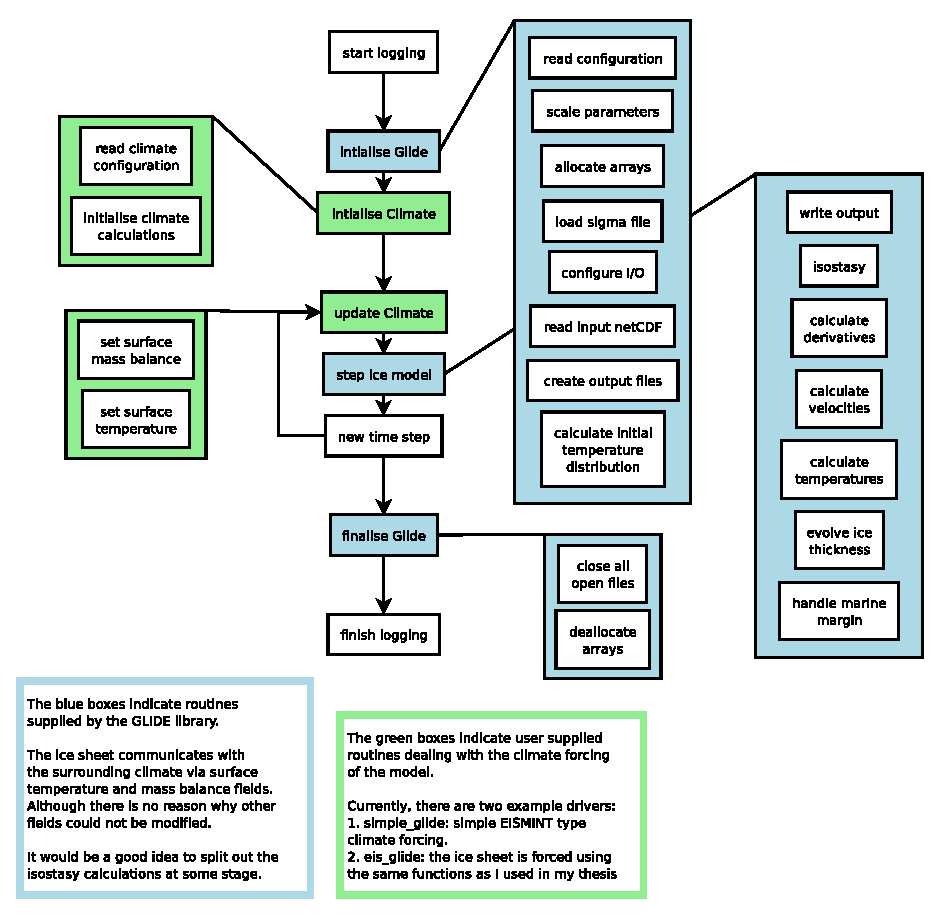
\epsfig{file=\dir/figs/glide.eps,width=0.9\textwidth}
 \end{center}
 \caption{Outline of the GLIDE and Climate components.}
\label{ug.glide}
\end{figure}

\subsection{Configuration, I/O and Visualisation}
Each component is configured using a configuration file similar to Windows \texttt{.ini} files. The model configuration is printed to a log file. 

2D and 3D data is read/written to netCDF files using the CF convention. netCDF is scientific data format for storing multidimensional data in a platform and language independent binary data format. The CF conventions specify the meta data used to describe the file contents.

Many programs can process and visualise netCDF data, e.g. OpenDX. Additionally, the GLIMMER module contains GMT scripts written in Python to visualise the output.

\subsection{Can I use GLIMMER with my climate model?}
We hope so! The external interface of GLIMMER is designed to be quite
flexible, but certain assumptions have necessarily been made about the form
taken by input fields, etc. Check out the climate drivers for examples of varying complexity.

\section{GLIMMER in practice -- an example}

\subsection{Initialising and calling}

The easiest way to learn how GLIMMER is used is by way of an
example. We assume that the GLIMMER code has been installed alongside the
climate model code, and can be compiled and linked successfully. Details of
how to achieve this may be found in the \texttt{COMPILE} file in the top-level
GLIMMER directory. 

Typically, GLIMMER will be called from the main program body of a
climate model. To make this possible, the compiler needs to be told to use the
GLIMMER code. Use statements appear at the very beginning of f90 program
units, before even \texttt{implicit none}:
%
\begin{verbatim}
  use glimmer_main
\end{verbatim}
%
The next task is to declare a variable of type \texttt{glimmer\_params}, which
holds everything relating to the model, including any number of ice-sheet
instances:
%
\begin{verbatim}
  type(glimmer_params) :: ice_sheet
\end{verbatim}
%
Before the ice-sheet model may be called from the climate model, it must be
initialised. This is done with the following subroutine call:
%
\begin{verbatim}
  call initialise_glimmer(ice_sheet,lats,lons,paramfile)
\end{verbatim}
%
In this call, the arguments are as follows:
%
\begin{itemize}
\item \texttt{ice\_sheet} is the variable of type \texttt{glimmer\_params}
 defined above;
\item \texttt{lats} and \texttt{lons} are one-dimensional arrays giving the
  locations of the global grid-points in latitude and longitude, respectively; 
\item \texttt{paramfile} is the file name of the top-level GLIMMER parameter
  namelist.
\end{itemize}
%
The contents of the namelist files will be dealt with later. Having
initialised the model, it may now be called as part of the main climate
model time-step loop:
%
\begin{verbatim}
    call glimmer(ice_sheet,time,temp,precip,zonwind,merwind,orog)
\end{verbatim} 
%
The arguments given in this example are the compulsory ones only; a number of
optional arguments may be specified -- these are detailed in the reference
section below. The compulsory arguments are:
%
\begin{itemize}
\item \texttt{ice\_sheet} is the variable of type \texttt{glimmer\_params}
 defined above;
\item \texttt{time} is the current model time, in years;
\item \texttt{temp} is the daily mean $2\,\mathrm{m}$ global air temperature field, in
  $^{\circ}\mathrm{C}$;
\item \texttt{precip} is the global daily precipitation fields,
  in $\mathrm{mm}/\mathrm{day}$ (water equivalent, making no distinction
  between rain, snow, etc.);
\item \texttt{zonwind} and \texttt{merwind} are the daily mean global zonal and
  meridional components of the $10\,\mathrm{m}$ wind field, in
  $\mathrm{ms}^{-1}$;
\item \texttt{orog} is the global orography field, in $\mathrm{m}$.
\end{itemize}
%
For the positive degree-day mass-balance routine, which is currently the only
mass-balance model included with GLIMMER, the daily quantities given above are
necessary, and, as such, GLIMMER should be called once per day. With the
energy and mass-balance model currently being developed, hourly calls will be
necessary. 
%
\subsection{Finishing off}
%
After the desired number of time-steps have been run, GLIMMER may have some
tidying up to do. To accomplish this, the subroutine \texttt{end\_glimmer}
must be called:
%
\begin{verbatim}
  call end_glimmer(ice_sheet)
\end{verbatim}
%

\subsection{Parameter Files}
\subsubsection{Format}
%
All parameter configuration files in GLIMMER use a custom, easily
understood file format, similar to Windows \texttt{.ini} files. The format is
described in full in section \ref{dg.sec.config_file}. 

Global parameters, applicable to all instances of the ice model are contained
in the file specified by \texttt{paramfile} in the call to
\texttt{initialise\_glimmer}. An example configuration file is given below (it is
the file \texttt{example.glp}):
%
\begin{verbatim}
[parameters]
time-step = 1.0
instance filenames:  g_land.gli
\end{verbatim}
%
The file contains only one section, \texttt{parameters}, which has two
name-value pairs: \texttt{time-step} and \texttt{instance filenames}. The
first of these is the main ice model time-step, in years. The second namelist
is a list of configuration files for each ice model instance. GLIMMER will
create ice model instances for each of the filenames listed here, without the
need to explicitly specify how many instances there are to be.

For each instance of the model, a configuration file with instance-specific
parameters must be supplied. The names of these files are given in the main
GLIMMER configuration file, as described above. The configuration file for an individual
instance is fairly long, so only a summary of the different sections
contained in it is given below. For an example this kind of file, see
\texttt{g\_land.gli} in the \texttt{data} directory.

Sections in an instance-specific file:
%
\begin{itemize}
\item \texttt{[output]} Configuration of model output -- contains the name of
  the configuration file controlling netCDF I/O. In the case of the example file
  \texttt{g\_land.gli}, the netCDF control file is \texttt{g\_land.glw}; see
  Section \ref{ug.sec.ncconf}. In addition, the file specified here also
  contains the name of the input file used (this will be changed in future).
\item \texttt{[domain size]} Model grid parameters -- number of grid points in $x$ and
  $y$ dimensions, and number of levels in the vertical.
\item \texttt{[projection]} Details of the projection used in the instance -- type of
  projection, and necessary parameters.
\item \texttt{[sigma coordinates]} -- contains the name of a
  sigma-coordinates file (see below)
\item \texttt{[options]} Flags specifying various model integration options, such
  as which of various schemes to use, etc.
\item \texttt{[time-steps]} The lengths of the various model time-steps
  relative to the main time-step.
\item \texttt{[grid-lengths]} The grid-lengths of the ice model domain.
\item \texttt{[parameters]} Physical parameters for the model, such as isostatic
  relaxation timescale.
\item \texttt{[forcing]} Parameters used by the forcing which may be used to run
  the model in stand-alone mode.
\item \texttt{[constants]} Constants used in the interface with the global
  model.
\item \texttt{[PDD scheme]} Parameters for the positive degree-day mass
  balance scheme.
\end{itemize}
%
\subsubsection{The Sigma coordinate file}
%
The name of the file containg the sigma variable is specified in
the instance-specific configuration file. This file consists of a
list of numbers in ascending order, between 0.0 and 1.0, specifying the
heights of the model levels in sigma space. The number of entries must be the
same as the number of model levels specified. An example file is
\texttt{g\_land.gls}.

\subsubsection{Grid I/O control files}
The model requires at least one field as input -- the height of the bedrock
topography (including bathymetry, if appropriate). If the bedrock is not in a relaxed state, then
the height of the relaxed topography must also be supplied. The bedrock is assumed to be relaxed 
if no relaxed topography field is supplied. Furthermore, the uppser surface of the ice sheet at the 
start of the run can be specified. These must be supplied as fields in a
netCDF file, whose name is given in the configuration file specified in the
\texttt{[output]} section of the main instance configuration file (see
above). A sample input file is supplied (\texttt{g\_land.input.nc}) - use
\texttt{ncdump} to determine the names of variables, dimensions and attributes.

Model output is controlled by the file listed in the \texttt{[output]} section
of the main instance-specific configuration file. Each model instance can save
specific variables to different netCDF files with different time intervals.
%
\subsection{Restarts}
%
{\bf N.B. GLIMMER does not currently have a functioning restart
  mechanism. This documentation is provided for information only at this stage.}

GLIMMER will provide two routines to handle restarts,
\texttt{glimmer\_write\_restart}, and \texttt{glimmer\_read\_restart}. The
former writes the entire model state to a single file, while the latter will
restore the model state from a previously created
file. For example, \texttt{glimmer\_write\_restart} may be called as follows:
%
\begin{verbatim}
  call glimmer_write_restart(ice_sheet,25,'ice_sheet.restart')
\end{verbatim}
%
Here, \texttt{ice\_sheet} is the GLIMMER parameter variable refered to
previously, \texttt{25} is the logical file-unit to use, and
\texttt{'ice\_sheet.restart'} is the filename of the restart file. This
subroutine call may be made at any point, regardless of whether it is intended
to halt the integration imminently, or not. In order to recover the model
state, the following call to \texttt{glimmer\_read\_restart} would be made:
%
\begin{verbatim}
  call glimmer_read_restart(ice_sheet,25,'ice_sheet.restart')
\end{verbatim}
%
The arguments are the same as for the previous call. When restarting from a
file like this, it is not necessary to make a call to
\texttt{initialise\_glimmer}. Note also that there is no alternative restart mechanism
provided within the normal \texttt{glimmer} subroutine call -- all restarts
must be called explicitly.

Note also that \texttt{glimmer\_read\_restart} may not be called if
\texttt{initialise\_glimmer} has been called already. This is because there is
currently no mechanism for \texttt{glimmer\_read\_restart} to know whether the
relevant model arrays have already been allocated. If they have, and
\texttt{glimmer\_read\_restart} tries to reallocate them, a fatal
run-time error will probably be generated. It is hoped to address this problem
in a future release.
%
\section{Namelist files}
%
This section contains information about the contents of the namelist files
used to configure GLIMMER.
%
\subsection{Top-level GLIMMER configuration file}
%
The top-level configuration file contains the following elements in the
following order:
\begin{center}
\begin{tabular}{l}
\texttt{timesteps} namelist \\
\texttt{file\_paras} namelist \\
List of instance-specific configuration files \\
\end{tabular}
\end{center}
%
\subsubsection {Possible \texttt{timesteps} namelist entry}
%
\begin{center}
\begin{tabular}{|c|c|c|l|}
\hline
Name & Type & Default & Description (units) \\
\hline
\hline
\texttt{tinc} & real & 1.0 & Main model time-step (years) \\
\hline
\end{tabular}
\end{center}
%
\subsubsection{Possible \texttt{file\_params} namelist entry}
\begin{center}
\begin{tabular}{|c|c|c|l|}
\hline
Name & Type & Default & Description (units) \\
\hline
\hline
\texttt{ninst} & integer & 1 & Number of ice model instances \\
\hline 
\end{tabular}
\end{center}
%
\subsubsection{List of instance-specific configuration files}
%
These filenames are given relative to the working directory of the climate
model. They must not be longer than 70 characters, though this may be altered
by changing the value of the parameter \texttt{fname\_length} in file
\texttt{glimmer\_global.f90}. The filenames should be given as plain text,
without quotation marks, and separated by newlines. 
%
\subsection{Instance-specific configuration files}
%
The instance-specific configuration files contain the following elements in
the following order:
\begin{center}
\begin{tabular}{l}
netCDF configuration file \\
\texttt{sizs} namelist \\
\texttt{prj} namelist \\
Name of sigma file \\
\texttt{opts} namelist \\
\texttt{nums} namelist \\
\texttt{pars} namelist \\
\texttt{dats} namelist \\
\texttt{cons} namelist \\
\texttt{forc} namelist \\
\end{tabular}
\end{center}
%
\subsubsection{netCDF configuration file}
%
As noted above, netCDF I/O is controlled by a separate configuration file. The configuration file is described on detail in Section \ref{ug.sec.ncconf}. Each model instance needs to be supplied with its own netCDF configuration file.
%
\subsubsection{Possible \texttt{sizs} namelist entries}
%
The \texttt{sizs} namelist specifies the model domain,
and may contain these elements:
%
\begin{center}
\begin{tabular}{|c|c|c|l|}
\hline
Name & Type & Default & Description (units) \\
\hline
\hline
\texttt{ewn} & integer & -- & Number of grid-points in the east-west
direction \\
\texttt{nsn} & integer & -- & Number of grid-points in the north-south
direction \\
\texttt{upn} & integer & 11 & Number of model levels \\
\hline
\end{tabular}
\end{center}
%
\subsubsection{Possible \texttt{prj} namelist entries}
%
The \texttt{prj} namelist specifies the parameters of the map projection, and
may contain these elements:
%
\begin{center}
\begin{tabular}{|c|c|c|l|}
\hline
Name & Type & Default & Description (units) \\
\hline
\hline
\texttt{p\_type} & integer & 1 & Type of projection: \\
 & & & 1) Lambert Equal Area \\
 & & & 2) Spherical polar \\
 & & & 3) Spherical stereographic (oblique) \\
 & & & 4) Spherical stereographic (equatorial) \\
\hline  
\texttt{lonc} & real & -- & Longitide of projection centre (degrees east) \\
\texttt{latc} & real & -- & Latitude of projection centre (degrees)\\
\texttt{cpx} & real & -- & Local $x$-coordinate of projection centre
(grid-points) \\
\texttt{cpy} & real & -- & Local $y$-coordinate of projection centre
(grid-points) \\
\hline
\end{tabular}
\end{center}
%
\subsubsection{Name of sigma file}
%
Conforms to the same rules as other filenames.
%
\subsubsection{Possible \texttt{opts} namelist entries}
%
The \texttt{opts} namelist specifies various ice model options, and may
contain these elements:
%
\begin{center}
    \tablefirsthead{%
    \hline
Name & Type & Default & Description (units)\\
    \hline
\hline}
  \tablehead{%
    \hline
    \multicolumn{4}{|p{0.98\textwidth}|}{\emph{\small continued from previous page}}\\
    \hline
Name & Type & Default & Description (units)\\
    \hline
\hline}
  \tabletail{%
    \hline
    \multicolumn{4}{|r|}{\emph{\small continued on next page}}\\
    \hline}
  \tablelasttail{\hline}


\begin{supertabular}{|c|c|c|p{8.5cm}|}
\texttt{whichtemp} & integer & 1 & {\raggedright
 Method of ice temperature calculation: \\
 \begin{tabular}{lp{7cm}}
  0 & Set column to surface air temperature \\
  1 & Do full temperature solution (also finds vertical velocity and apparent
  vertical velocity). \\
  2 & Set column to surface air temperature, but correct for melting-point
  effects. \\
 \end{tabular}}\\
\hline
\texttt{whichartm} & integer & 3 & {\raggedright
Method of calculation of surface air temperature:\\ 
 \begin{tabular}{lp{7cm}}
 0 & Linear function of surface elevation\\
 1 & Cubic function of distance from domain centre\\
 2 & Linear function of distance from domain centre\\
 3 & Greenland conditions (function of surface elevation and latitude) including forcing\\
 4 & Antarctic conditions (sea-level air temperature -- function of position)\\
 5 & Uniform temperature, zero range (temperature set in \texttt{cons} namelist) \\
 6 & Uniform temperature, corrected for height, zero range.\\
 7 & Use large-scale temperature and range.\\
 \end{tabular}}
\\
\hline
\texttt{whichthck} & integer & 4 & {\raggedright
Source of initial conditions: \\
\begin{tabular}{lp{7cm}}
1 & Read from file\\
2 & Set equal to one time-step of net accumulation (where positive)\\
3 & Stepped, linear function of distance from domain centre\\
4 & Read from file\\
5-7& Unknown\\
\end{tabular}}\\
\hline
\texttt{whichflwa} & integer & 0 & {\raggedright Method for calculating flow factor $A$:\\
\begin{tabular}{lp{7cm}}
0 & \emph{Patterson and Budd} relationship\\
1 & \emph{Patterson and Budd} relationship, with temperature set to $-10^{\circ}\mathrm{C}$ \\
2 & Set equal to $1\times 10^{-16}\,\mathrm{yr}^{-1}\,\mathrm{Pa}^{-n}$\\
\end{tabular}}\\
\hline
\texttt{whichisot} & integer & 1 & {\raggedright
Bedrock elevation: \\
\begin{tabular}{lp{7cm}}
0 & Fixed at input values\\
1 & Local function of ice loading history (ODE)\\
2 & Local function of ice loading history (ODE) with flexure\\
\end{tabular}}\\
\hline 
\texttt{whichslip} & integer & 4 & {\raggedright
Horizontal bed velocity: \\
\begin{tabular}{lp{7cm}}
0 & Linear function of gravitational driving stress\\
1-3 & Unknown\\
4 & Set to zero everywhere\\
\end{tabular}}\\
\hline
\texttt{whichbwat} & integer & 2 &{\raggedright
 Basal water depth: \\
\begin{tabular}{lp{7cm}}
0 & Calculated from local basal water balance\\
1 & as (0), including constant horizontal flow\\
2 & Set to zero everywhere\\
\end{tabular}}\\
\hline
\texttt{whichmarn} & integer & 0 &{\raggedright
 Ice thickness: \\
\begin{tabular}{lp{7cm}}
0 & Set thickness to zero if relaxed bedrock is more than certain water depth (??) \\
1 &  Set thickness to zero if floating \\
2 &  No action \\
\end{tabular}}\\
\hline
\texttt{whichbtrc} & integer & 1 & {\raggedright
Basal slip coefficient: \\
\begin{tabular}{lp{7cm}}
0 & \texttt{tanh} function of basal water depth\\
1 &  Set equal to zero everywhere\\
\end{tabular}}\\
\hline
\texttt{whichacab} & integer & 2 &{\raggedright
 Net accumulation: \\
\begin{tabular}{lp{7cm}}
0 & EISMINT moving margin \\
1 & PDD mass-balance model [recommended] \\
2 & Accumulation only\\
\end{tabular}}\\
\hline
\texttt{whichstrs} & integer & 2 & {\raggedright
Stress solution: \\
\begin{tabular}{lp{7cm}}
0 & Zeroth-order\\
1 & First-order\\
2 & Vertically-integrated first-order\\
3 & No action (use when velocity found elsewhere)\\
\end{tabular}}\\
\hline
\texttt{whichefvs} & integer & ? & ?? \\
\hline
\texttt{whichbabc} & integer & 0 &  {\raggedright Basal boundary condition? No options!}\\
\hline
\texttt{whichevol} & integer & 0 & {\raggedright
Thickness evolution method:\\
\begin{tabular}{lp{7cm}}
0 & Pseudo-diffusion approach \\
2 & Diffusion approach (also calculates velocities)\\
\end{tabular}}\\
\hline 
\texttt{whichwvel} & integer & 0 & Vertical velocities: \\
 & & & 0) Usual vertical integration \\
 & & & 1) Vertical integration constrained so that \\
 & & & upper kinematic B.C. obeyed \\
\hline 
\texttt{whichmask} & integer & 0 & ?? \\
\hline
\texttt{whichprecip} & integer & 0 & {\raggedright
Source of precipitation:\\
\begin{tabular}{lp{7cm}}
0 & Uniform precipitation rate (set internally at present)\\
1 & Use large-scale precipitation rate\\
2 & Use parameterization of \emph{Roe and Lindzen}\\
\end{tabular}}\\
\hline
\end{supertabular}
\end{center}
%
\subsubsection{Possible \texttt{nums} namelist entries}
%
\begin{center}
\begin{tabular}{|c|c|c|l|}
\hline
Name & Type & Default & Description (units)\\
\hline
\hline
\texttt{ntem}    & real & 1 & Length of temperature time-step as \\
 & & & a multiple of main timestep \\
\hline
\texttt{nvel}    & real & 1 & Length of velocity time-step as \\
 & & & a multiple of main time-step\\
\hline
\texttt{niso}    & real & 1 & Length of isostasy time-step as \\
 & & & a multiple of main time-step\\
\hline
\texttt{nout(3)} & real & (1,10,10) & Time between outputs for time-series, \\
 & & & 2D and 3D fields (years)\\
\hline
\texttt{nstr}    & real & & Start-time for 2D and 3D output (years) \\
\hline
\texttt{thklim} & real & 100 & Lower limit for 3D ice calculations (m?) \\
\hline
\texttt{mlimit} & real & -- & ? \\
\hline
\texttt{dew} & real & -- & Horizontal grid spacing in east-west direction (m)
\\
\hline
\texttt{dns} & real & -- & Horizontal grid spacing in north-south direction (m) \\
\hline
\end{tabular}
\end{center}
%
\subsubsection{Possible \texttt{pars} namelist entries}
%
\begin{center}
\begin{tabular}{|c|c|c|l|}
\hline
Name & Type & Default & Description (units)\\
\hline
\hline
\texttt{geot} & real & $-5\times 10^{-2}$ & Geothermal heat flux
($\mathrm{Wm}^{-2}$) \\
\hline
\texttt{fiddle} & real & 3.0 & Multiplier for flow factor \\
\hline
\texttt{airt(2)} & real & (-3.15,-0.01) & Air temperature parameterization
factors \\
 & & & (K, $\mathrm{K}\,\mathrm{km}^{-3}$) \\
\hline
\texttt{nmsb(3)} & real & (0.5, $1.05\times 10^{-5}$,  & Net accumulation
factors used in \\
 & & $4.5\times 10^{5}$) & combination with $\mathtt{whichthck}=2,3$ \\
 & & & ($\mathrm{m}\,\mathrm{yr}^{-1}$, $\mathrm{yr}^{-1}$, m) \\
\hline
\texttt{hydtim} & real & 1000 & 1) Basal hydrology time constant (When \\
 & & & $\mathtt{whichbwat}=0$) (yr)\\
 & & & 2) Basal hydrology advection velocity (When \\
 & & & $\mathtt{whichbwat}=1$) ($\mathrm{m}\,\mathrm{yr}^{-1}$)\\
\hline
\texttt{isotim} & real & 3000 & Isostasy time-constant (used in combination \\
 & & & with \texttt{whichisot} (yr) \\
\hline 
\texttt{bpar(5)} & real & (2.0, 10.0, 10.0, & Basal traction factors (used in \\
 & & 0.0, 1.0) & combination with \texttt{whichbtrc}). These describe the \\
 & & & form of the $B=\tanh(W)$ function: \\
 & & & (1) Width of tanh curve \\
 & & & (2) $W$ at midpoint of tanh curve (m) \\
 & & & (3) $B$ minimum ($\mathrm{m}\,\mathrm{yr}^{-1}\,\mathrm{Pa}^{-1}$) \\
 & & & (4) $B$ maximum ($\mathrm{m}\,\mathrm{yr}^{-1}\,\mathrm{Pa}^{-1}$) \\
 & & & (5) multiplier for marine sediments \\
\hline
\end{tabular}
\end{center}
%
\subsubsection{Possible \texttt{dats} namelist entries}
%
\begin{center}
\begin{tabular}{|c|c|c|l|}
\hline
Name & Type & Default & Description (units)\\
\hline
\hline
& & & \\
\hline
\end{tabular}
\end{center}
%
\subsubsection{Possible \texttt{cons} namelist entries}
%
\begin{center}
\begin{tabular}{|c|c|c|l|}
\hline
Name & Type & Default & Description (units)\\
\hline
\hline
\texttt{lapse\_rate} & real & -8.0 & Lapse rate used when adjusting \\
 & & & air temperature for elevation ($\mathrm{K}\,\mathrm{km}^{-1}$) \\
\hline
\texttt{precip\_rate} & real & 0.5 & Uniform precipitation rate,
\\
 & & & used in conjuction with \texttt{whichprecip}=0 \\
 & & & ($\mathrm{m}\,\mathrm{yr}^{-1}$ water equivalent) \\
\hline
\texttt{air\_temp} & real & -20.0 & Uniform surface air temperature, \\
 & & & used in conjunction with \texttt{whichsurftemp}=0,1 ($^{\circ}\mathrm{C}$) \\
\hline
\texttt{albedo} & real & 0.4 & Ice albedo \\
\hline
\end{tabular}
\end{center}
%
\subsection{Possible \texttt{forc} namelist entries}
%
\begin{center}
\begin{tabular}{|c|c|c|l|}
\hline
Name & Type & Default & Description (units)\\
\hline
\hline
\texttt{trun} & real & -- & Length of model run (years).\\
 & & & {\bf N.B.} This variable {\em does not} control the length of \\
 & & & the model run --- it is used in the case when \texttt{whichartm}=3 \\
 & & & to tell the forcing initialisation how long the run is going to be. \\
\hline
\end{tabular}
\end{center}
\section{Configuring netCDF I/O}\label{ug.sec.ncconf}
netCDF is a programming language and platform independent library used for managing multi--dimensional gridded data. There are many programs which can be used to processes and visualise netCDF data files.

GLIMMER netCDF output is controlled by a parameter file. Any number of input and output files can be specified. Metadata describing the numerical experiment can be attached. Empty lines and lines beginning with a \texttt{\#}, \texttt{;} or \texttt{!} are ignored.

\subsection{Metadata}
The metadata section \texttt{[default]} contains descriptions of the numerical experiment. The following parameter names are recognised:
\begin{center}
\begin{tabular}{|c|p{10cm}|}
\hline
Name & Description \\
\hline
\hline
\texttt{title}& Title of the experiment\\
\hline
\texttt{institution} & Institution at which the experiment was run\\
\hline
\texttt{references} & References that might be useful\\
\hline
\texttt{comment} & A comment, further describing the experiment\\
\hline
\end{tabular}
\end{center}
Any of these parameters can be modified in the \texttt{[output]} section (see \ref{ug.sec.nc_out}). The model automatically attaches a time stamp and the model version to the netCDF output file.

\subsection{Input}
The section controlling netCDF input is called \texttt{[input]}. Any number of input files can be specified. They are processed in the order they occur in the configuration file, potentially overriding previously loaded variables. The following parameter are recognised:
\begin{center}
\begin{tabular}{|c|p{10cm}|}
\hline
Name & Description \\
\hline
\hline
\texttt{name}& The name of the netCDF file to be read. Typically netCDF files end with \texttt{.nc}.\\
\hline
\texttt{time}& The time slice to be read from the netCDF file. The first time slice is read by default.\\
\hline
\end{tabular}
\end{center}
Only variables marked with $^\ast$ in Appendix \ref{ug.sec.varlist} are loaded.

\subsection{Output}\label{ug.sec.nc_out}
The \texttt{[output]} section of the netCDF parameter file controls how often selected  variables are written to file. The following parameter are recognised:
\begin{center}
\begin{tabular}{|c|p{10cm}|}
\hline
Name & Description \\
\hline
\hline
\texttt{name} & The name of the output netCDF file. Typically netCDF files end with \texttt{.nc}.\\
\hline
\texttt{frequency} & The time interval in years, determining how often selected variables are written to file.\\
\hline
\texttt{variables} & List of variables to be written to file. See Appendix \ref{ug.sec.varlist} for a list of known variables. Names should be separated by at least one space. The variable names are case sensitive. Append \texttt{\_spot} to the variable name to store variable at specified locations.\\
\hline
\texttt{numspot} & The number of spot locations\\
\hline
\texttt{spotx} & List of $x$--indecies specifying spot locations.\\
\hline
\texttt{spoty} & List of $y$--indecies specifying spot locations.\\
\hline
\end{tabular}
\end{center}

\section{GLIMMER subprogram calls}
%
This section details the subroutine calls provided by GLIMMER, and their
arguments. Note that where a type is given as \texttt{real(rk)}, this
indicates that the kind of the real type is specified by the value of
parameter \texttt{rk}, which may be altered in the file \texttt{glimmer\_globals.f90}.
%
\subsection{Subroutine \texttt{initialise\_glimmer}}
%
\paragraph{Purpose} To initialise the ice model, and load in all relevant parameter files.
%
\paragraph{Name and mandatory arguments}
%
\begin{verbatim}
  subroutine initialise_glimmer(params,lats,longs,paramfile)
\end{verbatim}
%
\paragraph{Arguments}
%
\begin{center}
\begin{tabular}{llll}
\texttt{params}    & \texttt{type(glimmer\_params)} & \texttt{intent(inout)} &
Ice model to be configured \\
\texttt{lats(:)}   & \texttt{real(rk)} & \texttt{intent(in)} & latitudinal location of grid-points in \\
 & & & global data (given in $^{\circ}\mathrm{N}$)\\
\texttt{longs(:)}  & \texttt{real(rk)} & \texttt{intent(in)} & longitudinal location of grid-points in \\
 & & & global data (given in $^{\circ}\mathrm{E}$)\\
\texttt{paramfile} & \texttt{character(*)} & \texttt{intent(in)} & name of
top-level GLIMMER \\
 & & & parameter file \\
\end{tabular}
\end{center}
%
\paragraph{Additional notes}
%
\begin{itemize}
\item The ice model determines the size of the global domain from the sizes of
  the arrays \texttt{lats} and \texttt{longs}.
\item The latitudes contained in \texttt{lats} must be in descending order, so
  that $\mathtt{lats(i)}>\mathtt{lats(i+1)}$ for $1\leq \mathtt{i} \leq
  \mathtt{size(lats)}$.
\end{itemize}
%
\subsection{Subroutine \texttt{glimmer}}
%
\paragraph{Purpose}
%
To perform temporal averaging of input fields, and, if necessary, down-scale
those fields onto local projections and perform an ice model time-step. Output
files may be appended to, and if optional arguments used, fields made
available for feedback.
%
\paragraph{Name and mandatory arguments}
%
\begin{verbatim}
  subroutine glimmer(params,time,temp,precip,zonwind,merwind,orog)
\end{verbatim}
%
\paragraph{Mandatory arguments}
%
\begin{center}
\begin{tabular}{llll}
\texttt{params} & \texttt{type(glimmer\_params)} & \texttt{intent(inout)} &
parameters for this run \\
\texttt{time} & \texttt{real(rk)} & \texttt{intent(in)} & Current model time
(hours) \\
\texttt{temp(:,:)} & \texttt{real(rk)} & \texttt{intent(in)} & Daily mean surface
temperature field ($^{\circ}\mathrm{C}$) \\
\texttt{precip(:,:)} & \texttt{real(rk)} & \texttt{intent(in)} & Daily
precipitation \\
 & & & field (mm/day) \\
\texttt{zonwind(:,:)} & \texttt{real(rk)} & \texttt{intent(in)} & Zonal
component of the wind field \\
 & & & ($\mathrm{ms}^{-1}$) \\
\texttt{merwind(:,:)} & \texttt{real(rk)} & \texttt{intent(in)} & Meridional 
component of the wind \\
 & & & field ($\mathrm{ms}^{-1}$) \\
\texttt{orog(:,:)} & \texttt{real(rk)} & \texttt{intent(in)} & Global orography (m) \\
\end{tabular}
\end{center}
%
\paragraph{Optional arguments}
%
\begin{center}
\begin{tabular}{llll}
\texttt{output\_flag} & \texttt{logical} & \texttt{intent(out)} & Set to show
new output fields have \\
 & & & been calculated after an ice-model time-step. \\
 & & & If this flag is not set, the output fields \\
 & & & retain their values at input. \\
\texttt{orog\_out(:,:)} & \texttt{real(rk)} & \texttt{intent(inout)} & Output
orography (m)\\ 
\texttt{albedo(:,:)} & \texttt{real(rk)} & \texttt{intent(inout)} & Surface
albedo \\
\texttt{ice\_frac(:,:)} & \texttt{real(rk)} & \texttt{intent(inout)} &
Fractional ice coverage \\
\texttt{fw\_flux(:,:)} & \texttt{real(rk)} & \texttt{intent(inout)} & The
fresh-water flux (mm/a) \\
 & & & This is simply the ablation calculated by the \\
 & & & model, scaled up to the global grid. It is up \\
 & & & to the global model to then  deal with it \\
 & & & (route it to the oceans, land scheme, etc.) \\
\end{tabular}
\end{center}
\paragraph{Additional notes}
%
\begin{itemize}
\item The sizes of all two-dimensional fields passed as arguments must be the
  same as that implied by the sizes of the arrays used to pass latitude and
  longitude information when the model was initialised using
  \texttt{initialise\_glimmer}. There is
  currently no checking mechanism in place for this, so using fields of the wrong size
  will lead to unpredictable results.
\item Zonal and meridional components of the wind are only required if the
  small-scale precipitation parameterization is being used (with
  \texttt{whichprecip} set to 2). In other circumstances, \texttt{zonwind} and
  \texttt{merwind} must still be arrays of the correct rank, but need not be
  the correct size, or may be unallocated if desired.
\item The optional output fields only refers to the parts of the globe
  covered by the GLIMMER ice model instances. The fraction of each global
  grid-box covered by ice model instances may be obtained using the
  \texttt{glimmer\_coverage\_map} subroutine below. 
\item The output orography field is given as a mean calculated over the part
  of the grid-box covered by ice  model instances. Thus, to calculate the
  grid-box mean, the output fields should be multiplied point-wise by the
  coverage fraction. 
\item Albedo is currently fixed at 0.4 for ice-covered ground, and set to zero
  elsewhere. The albedo is given for the part of the global grid box covered
  by ice, not as an average of the part covered by the ice model. No attempt
  is made to guess the albedo of the parts of the ice model domain \emph{not}
  covered by ice.
\end{itemize}
%
\paragraph{Example interpretation of output fields}
%
Consider a particular point, $(i,j)$ in the global domain. Suppose value
returned by \texttt{glimmer\_coverage\_map} for this point is 0.7, and the
output fields have these values:
\begin{verbatim}
  orog_out(i,j)  = 200.0
  albedo(i,j)    =   0.4
  ice_frac(i,j)  =   0.5
\end{verbatim}
%
What does this mean? Well, the ice model covers 70\% of the grid-box, and in
that part the mean surface elevation is 200\,m. Of the part covered by the ice
model, half is actually covered by ice. Thus, 35\% ($0.5\times 0.7$) of the global grid-box is
covered by ice, and the ice has an mean albedo of 40\%. The model makes no suggestion for the
albedo or elevation of the other 65\% of the grid-box.
%
\subsection{Subroutine \texttt{end\_glimmer}}
%
\paragraph{Purpose} To perform general tidying-up operations, close files, etc.
%
\paragraph{Name and mandatory arguments}
%
\begin{verbatim}
  subroutine end_glimmer(params)
\end{verbatim}
%
\paragraph{Arguments}
%
\begin{center}
\begin{tabular}{llll}
\texttt{params} & \texttt{type(glimmer\_params)} & \texttt{intent(inout)} & Ice model
parameters \\
\end{tabular}
\end{center}
%
\subsection{Function \texttt{glimmer\_coverage\_map}}
%
\paragraph{Purpose} To obtain a map of fractional coverage of global
grid-boxes by GLIMMER ice model instances. The function returns a value
indicating success, or giving error information.
%
\paragraph{Type, name and mandatory arguments}
%
\begin{verbatim}
  integer function glimmer_coverage_map(params,coverage)
\end{verbatim}
%
\paragraph{Arguments}
%
\begin{center}
\begin{tabular}{llll}
\texttt{params} & \texttt{type(glimmer\_params)} & \texttt{intent(in)} & Ice model parameters \\
\texttt{coverage(:,:)} & \texttt{real(rk)} & \texttt{intent(out)} & Coverage
map \\
\end{tabular}
\end{center}
%
\paragraph{Returned value}
%
\begin{center}
\begin{tabular}{|c|l|}
\hline
Value & Meaning \\
\hline
\hline
0 & Coverage map has been returned successfully \\
1 & Coverage map not yet calculated; must call \texttt{initialise\_glimmer}
first \\
2 & Array \texttt{coverage} is the wrong size \\
\hline
\end{tabular}
\end{center}
%
\subsection{Function \texttt{glimmer\_main\_funit}}
%
\paragraph{Purpose}
%
To return the value of the main logical file unit used by glimmer for writing
and reading files. This unit is used for all read/write operations except for
the glimmer log file (\texttt{glimmer.gll}), which uses a fixed unit (21). The
default value for the unit is 20, but this may be changed at any time, even
when the model is being run.
%
\paragraph{Type, name and mandatory arguments}
%
\begin{verbatim}
  integer glimmer_main_funit(params)
\end{verbatim}
%
\paragraph{Arguments}
%
\begin{center}
\begin{tabular}{llll}
\texttt{params} & \texttt{type(glimmer\_params)} & \texttt{intent(in)} & Ice model parameters \\
\end{tabular}
\end{center}
%
\paragraph{Returned value}
%
The returned value is the logical file unit being used.
%
\subsection{Subroutine \texttt{glimmer\_set\_main\_funit}}
%
\paragraph{Purpose}
%
To set the value of the logical file unit being used by glimmer for writing
and reading files. See previous entry for more details.
%
\paragraph{Name and mandatory arguments}
%
\begin{verbatim}
  glimmer_set_main_funit(params,unit)
\end{verbatim}
%
\paragraph{Arguments}
%
\begin{center}
\begin{tabular}{llll}
\texttt{params} & \texttt{type(glimmer\_params)} & \texttt{intent(inout)} &
Ice model parameters \\
\texttt{unit} & \texttt{integer} & \texttt{intent(in)} & Logical file unit to
be set \\
\end{tabular}
\end{center}
%
\subsection{Subroutine \texttt{glimmer\_write\_restart}}
%
\paragraph{Purpose}
%
To write a restart file containing the whole model state, including all ice
model instances and associated projection data.
%
\paragraph{Name and mandatory arguments}
%
\begin{verbatim}
  glimmer_write_restart(params,unit,filename)
\end{verbatim}
%
\paragraph{Arguments}
%
\begin{center}
\begin{tabular}{llll}
\texttt{params} & \texttt{type(glimmer\_params)} & \texttt{intent(in)} &
Ice model parameters \\
\texttt{unit} & \texttt{integer} & \texttt{intent(in)} & Logical file unit to
use \\
\texttt{filename} & \texttt{character(*)} & \texttt{intent(in)} & Filename to
write \\
\end{tabular}
\end{center}
%
\subsection{Subroutine \texttt{glimmer\_read\_restart}}
%
\paragraph{Purpose}
%
To read a restart file containing the whole model state, including all ice
model instances and associated projection data.
%
\paragraph{Name and mandatory arguments}
%
\begin{verbatim}
  glimmer_read_restart(params,unit,filename)
\end{verbatim}
%
\paragraph{Arguments}
%
\begin{center}
\begin{tabular}{llll}
\texttt{params} & \texttt{type(glimmer\_params)} & \texttt{intent(out)} &
Ice model parameters \\
\texttt{unit} & \texttt{integer} & \texttt{intent(in)} & Logical file unit to
use \\
\texttt{filename} & \texttt{character(*)} & \texttt{intent(in)} & Filename to
read \\
\end{tabular}
\end{center}




\chapter{Tutorial}
\renewcommand{\dir}{tut}
\section{Introduction}
Ice sheet dynamics are fairly well understood and, thus, models simulating ice sheet physics are fairly standard. Ice sheet models are now used as part of larger Earth System Models or as the model core to investigate interactions with their surroundings such as basal erosion. 

GLIMMER\footnote{GLIMMER used to be an acronym the meening of which has long been lost. It should no be considered to be a nice name.} is a set of libraries, utilities and example climate drivers used to simulate ice sheet evolution. Its design is motivated by the desire to create an ice modelling system which is easy to interface to a wide variety of climate models, without the user having to have a detailed knowledge of its inner workings. This is accomplished by providing a very well-defined interface, which allows access to all the functionality required by the user.

\subsection{Overview}
GLIMMER consists of
\begin{enumerate}
\item {\bf GLIDE:} {\bf G}eneral {\bf L}and {\bf I}ce {\bf D}ynamic {\bf E}lements, the core of the model.  This component is the actual ice sheet model. GLIDE is responsible for calculating ice velocities, internal ice temperature distribution, isostatic adjustment and melt water production.
\item {\bf SIMPLE:} EISMINT climate drivers.
\item {\bf GLINT:} {\bf G}ENIE {\bf I}nterface. Coupler for the GENIE\footnote{Grid-ENabled Integrated Earth-system model} Earth Systems Model.
\item {\bf EIS:} {\bf E}dinburgh {\bf I}ce {\bf S}heet climate driver based on a parameterisation of the equilibrium line altitude, sea--level surface temperatures and eustatic sea--level change.
\item {\bf GLUM:} {\bf G}Limmer {\bf U}seful {\bf M}odules, various utility procedures used by the other components.
\item Visualisation programs using GMT\footnote{Generic Mapping Tools}.
\end{enumerate}
\begin{figure}[htbp]
  \centering
  \epsfig{file=\dir/figs/glimmer.eps,width=0.6\textwidth}
  \caption{Relationship between the various GLIMMER components.}
  \label{ug.fig.glimmer}
\end{figure}
The relationship between the GLIMMER components is illustrated in Figure \ref{ug.fig.glimmer}.


\subsection{What are `Multiply Enabled Regions'?}
The most distinctive feature of the GLIMMER framework is the ability to run different \emph{instances} of the ice model. These instances can be different regions of the globe and/or different sets of model parameters. Currently, this feature is only used by the GLINT climate driver which handles the processes of downscaling input variables, and subsequently aggregating and upscaling outputs.

\subsection{Climate Drivers}
The core ice sheet model, GLIDE, is connected to the climate via the surface mass balance and temperature fields and (optionally) a scalar value for eustatic sea level. These drivers can be derived from simple assumptions, e.g. uniform mass balance or EISMINT tests, or from climate model output, e.g. GENIE or a regional climate model. These components and how their relations are outlined in Figure \ref{ug.glide}.

\begin{figure}[htbp]
 \begin{center}
   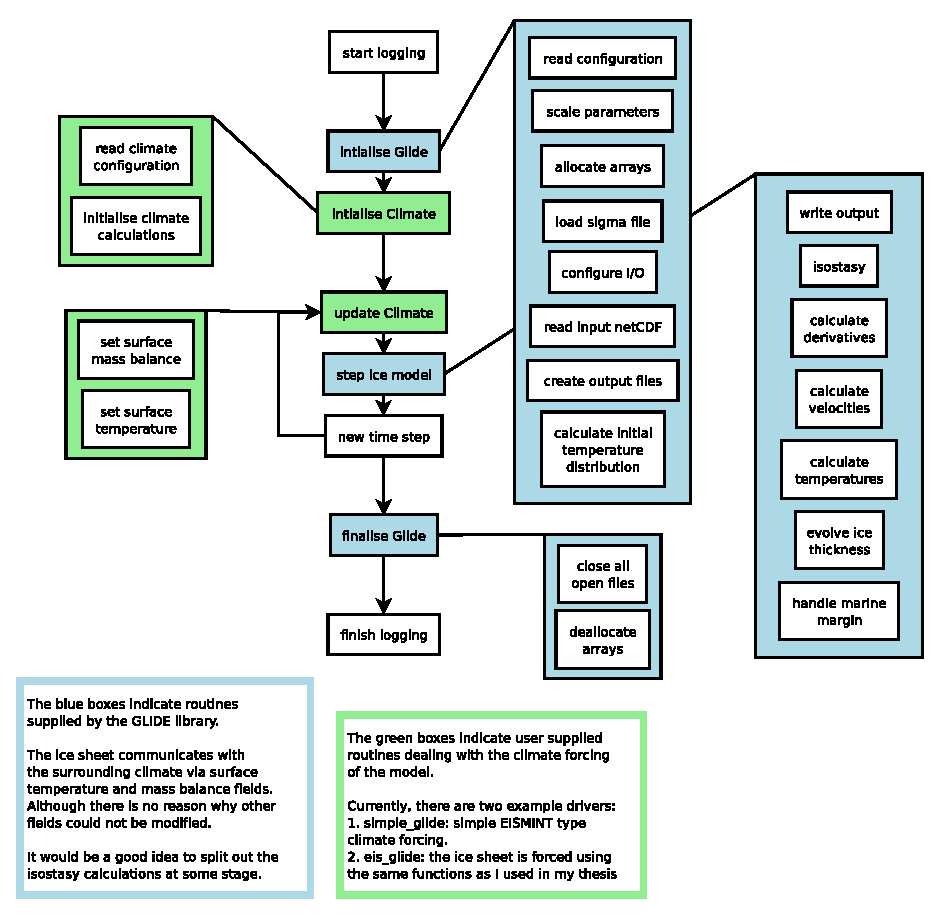
\epsfig{file=\dir/figs/glide.eps,width=0.9\textwidth}
 \end{center}
 \caption{Outline of the GLIDE and Climate components.}
\label{ug.glide}
\end{figure}

\subsection{Configuration, I/O and Visualisation}
Each component is configured using a configuration file similar to Windows \texttt{.ini} files. The model configuration is printed to a log file. 

2D and 3D data is read/written to netCDF files using the CF convention. netCDF is scientific data format for storing multidimensional data in a platform and language independent binary data format. The CF conventions specify the meta data used to describe the file contents.

Many programs can process and visualise netCDF data, e.g. OpenDX. Additionally, the GLIMMER module contains GMT scripts written in Python to visualise the output.

\subsection{Can I use GLIMMER with my climate model?}
We hope so! The external interface of GLIMMER is designed to be quite
flexible, but certain assumptions have necessarily been made about the form
taken by input fields, etc. Check out the climate drivers for examples of varying complexity.


\section{EISMINT: using \texttt{glimmer-example}}
As you hopefully already know, the heart of GLIMMER is the actual ice sheet model
GLIDE. This is where ice physics are resolved etc. To model an ice sheet using
GLIDE, you at least need to provide it with information about the 
mass balance. To get you started with a real simple example climate driver,
download \texttt{glimmer-example} from the project homepage or via CVS, cd into
the directory and type
\begin{verbatim}
glide_launch.py example.config
\end{verbatim}
this will kick off a simple EISMINT-1 moving margin type model run. The results
are written to \texttt{example.nc}, use a viewer like ncview to visualise them.
Take a look at the \texttt{example.config} file printed below and read the documentation on
the EISMINT type climate driver (section \ref{driver:eismint}) to better understand what is happening:\\

\begin{verbatim}
# configuration for the EISMINT-1 test-case # moving margin

[EISMINT-1 moving margin]

[grid]
# grid sizes
ewn = 31
nsn = 31
upn = 11
dew = 50000
dns = 50000

[options]
temperature = 1
flow_law = 2
isostasy = 0
sliding_law = 4
marine_margin = 2
stress_calc = 2
evolution = 2
basal_water = 2
vertical_integration = 0

[time]
tend = 200000.
dt = 10.
ntem = 1.
nvel = 1.
niso = 1.

[parameters]
flow_factor = 1
geothermal = -42e-3

[CF default]
title: EISMINT-1 moving margin

[CF output]
name: example.nc
frequency: 1000
variables: thk uflx vflx bmlt temp
uvel vvel wvel
\end{verbatim}

The line \texttt{[EISMINT-1 moving margin]} sets the model type for this run to be EISMINT (simple_glide binary).
This can also be achieved by specifying the correct binary using the \texttt{-m} flag, e.g.
\begin{verbatim}
glide_launch.py -m simple_glide example.config
\end{verbatim}
It is probably advisable to use the \texttt{-m} option instead of specifying the binary using a 
keyterm, as this will only work for EIS and EISMINT model types. For ease of use, the option was integrated
in the config file for this example. 

The \texttt{[grid]} section sets up the topography for the model run.\\
As this is an EISMINT testcase, there is no 'real' input topography, but ice is building up on a
flat surface, which is why nothing more but the grid dimensions need to be specified. Be aware that
this only works for EISMINT type model runs using simple\_glide.
In this case, the mass balance is parameterised as a function of distance
from the grid center, resulting in a point symmetric ice sheet.
The grid used here has a size of 31x31 cells (\texttt{ewn x
nsn}), comprises of 11 vertical layers (\texttt{upn = 11}) and an internal cell spacing of
5000 (\texttt{dew} and \texttt{dns}).

The \texttt{[options]} sections determines the basic behaviour of the model:\\
\texttt{temperature = 1} resolves the temperature over the whole of the 11
layers of ice (instead of assuming ice to be isothermal), \texttt{isostasy = 0}
turns off the isostasy component, etc. (check the documentation).

In the \texttt{[time]} section, the end time of the model run is set to 200000
with a timestep size of 10 and keeping all internal update processes
(temperature and velocity) in line with the timesteps by setting their
multiplier to 1.

Flow factor and geothermal heat flux parameters are set in the
\texttt{[parameters]} section.

Finally, in the \texttt{[CF output]} section, the name of the file to store the results
is given, together with the \texttt{variables} that should be dumped to the file and the
\texttt{frequency} with which they are written to it (every 1000 years). In this example, 
ice thickness (\texttt{thk}), basal melt temperature \texttt{bmlt}, ice temperature \texttt{temp} etc 
is output to the result file every 1000 years. Note that this output frequency is independent of the
modelling timesteps.

You might want to try and change some of the parameters, e.g. speed up ice flow by 
increasing the flow factor, and re-run the model to see what happens.
This is fairly simple and straight forward example of how to get GLIMMER to do some 
basic modelling. If you want to see a bit more of what GLIMMER can do, try the next section.


\section{EIS: using \texttt{glimmer-tests}}
\texttt{glimmer-tests} provides more example configurations, that include both the EISMINT
and EIS climate drivers. If you have not already done so, download
\texttt{glimmer-tests} via the nescforge page or CVS, and do the usual
\begin{verbatim}
    ./configure -with-glimmer-prefix=/path/to/Glimmer/installation
    (e.g. /usr/local/glimmer)
\end{verbatim}
(if you updated Glimmer via CVS, you need to do \texttt{./bootstrap} first.)\\
\texttt{glimmer-tests} is not (yet) a test suite, but will exemplarily show
what Glimmer can do (see the \texttt{glimmer-tests} README file for detailed
information on the tests).

Basically \texttt{glimmer-tests} runs Glimmer using the EISMINT 1 and 2 (and 3)
climate driver (fixed and moving margin type ice sheets with no external mass
balance forcing), as well as the Edinburgh Ice Sheet (EIS) climate driver,
using mass balance parameterisation via ELA and temperature forcing. There are
a couple of other tests running besides this, e.g. some benchmarks. If you want
to run all the examples, simply do a \texttt{make} in the
\texttt{glimmer-tests} directory, but be aware that running all tests will take a good
12+ hours on a single CPU 3 GHZ machine. If you're too impatient for this,
simply do a \texttt{make} in one of the subdirectories, e.g. EISMINT1 and GLIDE
will be launched using the EISMINT climate driver, which should deliver you a
number of netcdf files with the model results, eg. \texttt{e1.fm.1.nc}
containing the EISMINT1 fixed margin results 1, etc. Again, to visualise the
results use a viewer like ncview.

If you want a more sophisticated results, try \texttt{make} in the \texttt{eis}
directory, which will repeat the results of \cite{Hagdorn2003} reconstructing
the Fennoscandian ice sheet during the last glacial maximum, using the EIS
driver.

\subsection{A short introduction to the EIS driver parameterisation}

Again, check the config file \texttt{fenscan.config} to see the basic
parameters for this model run. Have a look at the \texttt{mb2.data} (mass
balance forcing via ELA), \texttt{temp-exp.model} (exponential type temperature
forcing) and \texttt{specmap.data} (sealevel change) data files and compare
them to the EIS driver documentation (section \ref{driver:eis}) to get an idea of how things are done.

The first column in every data file is the model time at which the new
parameter values are applied. For the temperature model, the records in the
\texttt{temp-exp.model} file
\begin{verbatim}
...
 -97000.000000  -17.858964  23.158964   -0.051329
 -96000.000000  -20.074036  24.674036   -0.051329
...
\end{verbatim}

correspond to the timesteps -97000 and -96000 (first column - model usually
ends at time 0) where the parameters a0 (2nd column), a1 (3rd column) and a2
(last column) of the exponential temperature model $T(t)=a_0+a_1\exp\left(a_2(\lambda-\lambda_0)\right)$
(page \pageref{driver:eis})
are updated to reflect an approximate change in temperature of -2 degrees
Celsius.

For EIS, the mass balance is parameterised via the ELA, according to
$$z_{\text{ELA}} = a + b\lambda + c\lambda^2 + \Delta z_{\text{ELA}},$$
given the parameters in the according config file section:
\begin{verbatim}
...
[EIS ELA]
ela_file = mb2.data
bmax_mar = 4.
ela_a = 14430.069930
ela_b =-371.765734
ela_c = 2.534965
...
\end{verbatim}
Factors a, b and c are specified together with the maximum mass balance of 4. The
latitude $\lambda$ in degrees North is read from the input topography grid. In
order to do the ELA forcing over time, the parameter $\Delta z_{ELA}$ is varied
over time using the ela file \texttt{mb2.data}:
\begin{verbatim}
...
 -109000 225
 -105000 350
...
\end{verbatim}

Similar to the temperature forcing, $\Delta z_{ELA}$ (column 2) is changed at
timestep -10900 (column 1), to reflect an ELA 225m above the altitude value
calculated using the factors a, b, c and the latitude $\lambda$. At timestep
-10500, ELA is rising to 350m above the calculated value.

Where a globally changing $\Delta z_{ELA}$ is insufficient to reflect
disparities in ELA, there are two options to fine tune ELA behaviour. First,
continentality can be used to introduce a dependency of mass balance with
distance to oceans. The according settings are supplied using the \texttt{[EIS CONY]}
section of the config file (see section \ref{driver:eis}).
In short, an index is calculated for every grid cell reflecting 
the ratio of below sealevel cells to land cells within a certain \texttt{range} (defaults to 600km).
Maximum mass balance values are then scaled between the values given in the \texttt{[EIS ELA]} section 
for \texttt{bmax\_mar} (marine conditions, all cells within \texttt{range} are below sea level) and
\texttt{bmax\_cont} (continenal conditions, all cells within \texttt{range} are above sea level).
Alternatively, continentality values between 0 and 1 can be input using a file. Set the according
flag \texttt{file} to 1 and specify the file containing the cony data using a \texttt{[CF input]} section
in the configuration file (see example for ELA file below).
.

In case a more detailed spatial distribution of ELA altitudes is needed, e.g. 
to reflect special orographic effects, a map of $\Delta z_{ELA}$ can be input
to the model using a netcdf file, containing a variable 'ela' on a grid
the same size and coordinates as the input topography grid the model is running
on. This ela file is coupled using a \texttt{[CF input]} section in the
configuration file
\begin{verbatim}
[CF input]
name: ela_1k.nc
\end{verbatim}
resulting in a spatial distribution of $\Delta z_{ELA}$ being applied to the
model. The variation of ELA over time using a global $\Delta z_{ELA}$ is still
applied on top of this ELA forcing file.

\textcolor[rgb]{1.00,0.00,0.00}{\emph{Note: (Maybe an example
containing an ELA forcing file should be added to Glimmer test/examples?)}}
\\
Sealevel changes are forced upon the model in an according way using the
\texttt{specmap.data} file.

\newpage
\subsection{GLINT driver}
\subsubsection{Overview}
%
GLINT is the most complex of the drivers supplied as part of GLIMMER. It was
originally developed as an interface between GLIDE and the GENIE Earth-system
model, but is designed to be flexible enough to be used with a wide range of
global climate models. Perhaps the most distinctive feature of GLINT is the
way it uses the object-oriented GLIDE architecture to enable multiple ice
models to be coupled to the same climate model. The means that regional ice
models can be run at high resolution over several parts of the globe, but
without the expense of running a global ice model.

GLINT automates the processes required in coupling regional models to a global
model, particularly the down- and up-scaling of the fields that form the
interface between the two models. The user may specify map projection
parameters for each of the ice models (known as \emph{instances}), and choose
one of several alternative mass-balance schemes to use in the coupling. The
differing time-steps of global model, mass-balance scheme, and ice model are
handled automatically by temporal averaging or accumulation of quantities (as
appropriate). This is illustrated schematically in figure~\ref{ug.fig.glint_timesteps}.  
%
\begin{figure}[htbp]
  \centering
  \includegraphics[width=0.6\textwidth]{\dir/figs/glint_timesteps.eps}
  \caption{Relationship between the timesteps in GLINT. The filled circles
  represent timesteps, the rectangles represent averaging/accumulation, and the arrows,
  flow of coupling fields.}
  \label{ug.fig.glint_timesteps}
\end{figure}
%
\subsubsection{Prerequisites}
%
In order to use GLIMMER, the following should be borne in mind:
%
\begin{itemize}
\item Global input fields must be supplied on a latitude-longitude
  grid. The grid does not have to be uniform in latitude, meaning that
  Gaussian grids may be used. Irregular grids (e.g. icosahedral grids) are not
  supported currently. The boundaries of the grid boxes may be specified; if
  not, they are assumed to lie half-way between the grid-points in lat-lon space.
\item In the global field arrays, latitude must be indexed from north to south
  -- i.e. the first row of the array is the northern-most one. Again, some
  flexibility might be introduced into this in the future.
\item The global grid must not have grid points at either of the
  poles. This restriction is not expected to be permanent, but in the meantime
  can probably be overcome by moving the location of the polar points to be
  fractionally short of the pole (e.g. at 89.9$^{\circ}$ and -89.9$^{\circ}$).
\end{itemize}
%
\subsubsection{Initialising and calling}

The easiest way to learn how GLINT is used is by way of an
example. GLINT should be built automatically as part of GLIMMER, and we assume
here that this has been achieved successfully.

Typically, GLINT will be called from the main program body of a
climate model. To make this possible, the compiler needs to be told to use the
GLINT code. Use statements appear at the very beginning of f90 program
units, before even \texttt{implicit none}:
%
\begin{verbatim}
  use glint_main
\end{verbatim}
%
The next task is to declare a variable of type \texttt{glint\_params}, which
holds everything relating to the model, including any number of ice-sheet
instances:
%
\begin{verbatim}
  type(glint_params) :: ice_sheet
\end{verbatim}
%
Before the ice-sheet model may be called from the climate model, it must be
initialised. This is done with the following subroutine call:
%
\begin{verbatim}
  call initialise_glint(ice_sheet,lats,lons,paramfile)
\end{verbatim}
%
In this call, the arguments are as follows:
%
\begin{itemize}
\item \texttt{ice\_sheet} is the variable of type \texttt{glint\_params}
 defined above;
\item \texttt{lats} and \texttt{lons} are one-dimensional arrays giving the
  locations of the global grid-points in latitude and longitude, respectively; 
\item \texttt{paramfile} is the name of the GLINT configuration file.
\end{itemize}
%
The contents of the namelist files will be dealt with later. Having
initialised the model, it may now be called as part of the main climate
model time-step loop:
%
\begin{verbatim}
    call glint(ice_sheet,time,temp,precip,zonwind,merwind,orog)
\end{verbatim} 
%
The arguments given in this example are the compulsory ones only; a number of
optional arguments may be specified -- these are detailed in the reference
section below. The compulsory arguments are:
%
\begin{itemize}
\item \texttt{ice\_sheet} is the variable of type \texttt{glint\_params}
 defined above;
\item \texttt{time} is the current model time, in hours;
\item \texttt{temp} is the daily mean $2\,\mathrm{m}$ global air temperature field, in
  $^{\circ}\mathrm{C}$;
\item \texttt{precip} is the global daily accumulated precipitation field,
  in $\mathrm{mm}$ (water equivalent, making no distinction
  between rain, snow, etc.);
\item \texttt{zonwind} and \texttt{merwind} are the daily mean global zonal and
  meridional components of the $10\,\mathrm{m}$ wind field, in
  $\mathrm{ms}^{-1}$;
\item \texttt{orog} is the global orography field, in $\mathrm{m}$.
\end{itemize}
%
For the positive degree-day mass-balance routine, which is currently the only
mass-balance model included with GLINT, the daily quantities given above are
necessary, and, as such, GLINT should be called once per day. With the
energy-balance mass-balance model currently being developed in the RAPID
project, hourly calls will be necessary. 
%
\subsubsection{Finishing off}
%
After the desired number of time-steps have been run, GLINT may have some
tidying up to do. To accomplish this, the subroutine \texttt{end\_glint}
must be called:
%
\begin{verbatim}
  call end_glint(ice_sheet)
\end{verbatim}
%
\subsubsection{API}
%
A detailed description of the GLINT API may be found in the appendices.
%
\subsubsection{Configuration}
%
GLINT uses the same configuration file format as the rest of GLIMMER. In the
case where only one GLIDE instance is used, all the configuration data for
GLINT and GLIDE can reside in the same file. Where two or more instances are
used, a top-level file specifies the number of model instances and the name of
a configuration file for each one. Possible configuration sections specific to
GLINT are as follows:
\begin{center}
  \tablefirsthead{%
    \hline
  }
  \tablehead{%
    \hline
    \multicolumn{2}{|p{0.98\textwidth}|}{\emph{\small continued from previous page}}\\
    \hline
  }
  \tabletail{%
    \hline
    \multicolumn{2}{|r|}{\emph{\small continued on next page}}\\
    \hline}
  \tablelasttail{\hline}
  \begin{supertabular}{|l|p{11cm}|}
%%%% 
    \hline
    \multicolumn{2}{|l|}{\texttt{[GLINT]}}\\
    \hline
    \multicolumn{2}{|p{0.98\textwidth}|}{Section specifying number of instances.}\\
    \hline
    \texttt{n\_instance} & (integer) Number of instances (default=1)\\
    \hline
%%%% 
    \hline
    \multicolumn{2}{|l|}{\texttt{[GLINT instance]}}\\
    \hline
    \multicolumn{2}{|p{0.98\textwidth}|}{Specifies the name of an
    instance-specific configuration file. Unnecessary if we only have one
    instance whose configuration data is in the main config file.}\\
    \hline
    \texttt{name} & Name of instance-sepcific config file (required).\\
    \hline
%%%% 
    \hline
    \multicolumn{2}{|l|}{\texttt{[GLINT projection]}}\\
    \hline
    \multicolumn{2}{|p{0.98\textwidth}|}{Projection info}\\
    \hline
    \texttt{projection} & {\raggedright (integer) type of projection:\\
       \begin{tabular}{lp{10cm}}
         1 & Lambert Equal Area \\
         2 & Spherical polar \\
         3 & Spherical stereographic (oblique)\\
         4 & Spherical stereographic (equatorial)\\
       \end{tabular}}\\
    \texttt{lonc} & Longitide of projection centre (degrees east)\\
    \texttt{latc} & Latitude of projection centre (degrees north)\\
    \texttt{cpx} & Local $x$-coordinate of projection centre (grid-points)\\
    \texttt{cpy} & Local $y$-coordinate of projection centre (grid-points)\\
    \texttt{std parallel} & Standard parallel of projection (degrees
    north). Only relevant when \texttt{projection}=3 (default=90.0)\\
    \texttt{earth\_radius} & Radius of the Earth (m) (default=$6.37\times10^6$)\\
    \hline
%%%% 
    \hline
    \multicolumn{2}{|l|}{\texttt{[GLINT climate]}}\\
    \hline
    \multicolumn{2}{|p{0.98\textwidth}|}{GLINT climate configuration}\\
    \hline
    \texttt{precip\_mode} & {\raggedright
      Method of precipitation downscaling: \\
      \begin{tabular}{lp{10cm}}
        {\bf 1} & Use large-scale precipitation rate\\
        2 & Use parameterization of \emph{Roe and Lindzen}\\
      \end{tabular}}\\
    \texttt{acab\_mode} & {\raggedright
      Mass-balance model to use:\\
      \begin{tabular}{lp{7cm}}
        {\bf 1} & Annual PDD mass-balance model (see section \ref{ug.mbal.pdd_scheme}) \\
        2 & Annual accumulation only\\
        3 & Hourly energy-balance model (RAPID - not yet available) \\
        4 & Daily PDD mass-balance model (no docs yet)\\
      \end{tabular}}\\
    \texttt{ice\_albedo} & Albedo of ice --- used for coupling to climate
    model (default=0.4) \\
    \texttt{lapse\_rate} & Atmospheric temperature lapse-rate, used to correct
    the atmospheric temperature onto the ice model orography. This should be
    \emph{positive} for temperature falling with height
    ($\mathrm{K}\,\mathrm{km}^{-1}$) (default=8.0) \\
    \hline
  \end{supertabular}
\end{center}



\part{Developer Documentation}

\chapter{Numerics}
\renewcommand{\dir}{num}
This part describes the numerical implementation of GLIMMER in some detail. It is hoped that more parts will be added in the future.
\section{Ice Thickness Evolution}
The evolution of the ice thickness, $H$, stems from the continuity equation and can be expressed as
\begin{equation}
  \label{kin.eq.ice_thickness}
  \frac{\pd H}{\pd t} = -\vec\nabla\cdot(\overline{\vec{u}} H) + B,
\end{equation}
where $\overline{\vec{u}}$ is the vertically averaged ice velocity, $B$ is the surface mass balance and $\vec\nabla$ is the horizontal gradient operator \citep{Payne1997}. 

For large--scale ice sheet models, the \emph{shallow ice approximation} is generally used. This approximation states that bedrock and ice surface slopes are assumed sufficiently small so that the normal stress components can be neglected \citep{Hutter1983}. The horizontal shear stresses ($\tau_{xz}$ and $\tau_{yz}$) can thus be approximated by
\begin{equation}
  \label{kin.eq.horiz_shear}
  \begin{split}
    \tau_{xz}(z)&=-\rho g(s-z)\frac{\pd s}{\pd x},\\
    \tau_{yz}(z)&=-\rho g(s-z)\frac{\pd s}{\pd y},
  \end{split}
\end{equation}
where $\rho$ is the density of ice, $g$ the acceleration due to gravity and $s=H+h$ the ice surface.

Strain rates $\dot{\epsilon}_{ij}$ of polycrystalline ice are related to the stress tensor by the non--linear flow law:
\begin{equation}
  \label{kin.eq.flowlaw}
  \dot{\epsilon}_{iz}=\frac12\left(\frac{\pd u_i}{\pd z}+\frac{\pd u_z}{\pd i}\right)=A(T^\ast)\tau_\ast^{(n-1)}\tau_{iz}\qquad i=x,y,
\end{equation}
where $\tau_\ast$ is the effective shear stress defined by the second invariant of the stress tensor, $n$ the flow law exponent and $A$ the temperature--dependent flow law coefficient. $T^\ast$ is the absolute temperature corrected for the dependence of the melting point on pressure \cite[$T^\ast=T+8.7\cdot10^{-4}(H+h-z)$, $T$ in Kelvin,][]{Huybrechts1986}. The parameters $A$ and $n$ have to be found by experiment. $n$ is usually taken to be 3. $A$ depends on factors such as temperature, crystal size and orientation, and ice impurities. Experiments suggest that $A$ follows the Arrhenius relationship:
\begin{equation}
  \label{kin.eq.arrhenius}
  A(T^\ast)=fae^{-Q/RT^\ast},
\end{equation}where $a$ is a temperature--independent material constant, $Q$ is the activation energy for creep and $R$ is the universal gas constant \citep{Paterson1994}. $f$ is a tuning parameter used to `speed--up' ice flow and accounts for ice impurities and the development of anisotropic ice fabrics \citep{Payne1999,Tarasov1999,Tarasov2000,Peltier2000}.

Integrating \eqref{kin.eq.arrhenius} with respect to $z$ gives the horizontal velocity profile:
\begin{equation}
  \label{kin.eq.horiz_velo}
  \vec u(z)-\vec u(h) = -2(\rho g)^n|\vec\nabla s|^{n-1}\vec\nabla s\int_h^zA(s-z)^ndz,
\end{equation}
where $\vec u(h)$ is the basal velocity (sliding velocity). Integrating \eqref{kin.eq.horiz_velo} again with respect to $z$ gives an expression for the vertically averaged ice velocity:
\begin{equation}
  \label{kin.eq.avg_velo}
  \overline{\vec u}H=-2(\rho g)^n|\vec\nabla s|^{n-1}\vec\nabla s\int_h^s\int_h^zA(s-z)^ndzdz'.
\end{equation}

The vertical ice velocity stems from the conservation of mass for an incompressible material:
\begin{equation}
  \label{kin.eq.incompress}
  \frac{\pd u_x}{\pd x} + \frac{\pd u_y}{\pd y} + \frac{\pd u_z}{\pd z} = 0.
\end{equation}
Integrating \eqref{kin.eq.incompress} with respect to $z$ gives the vertical velocity distribution of each ice column:
\begin{equation}
  \label{kin.eq.vert_velo}
  w(z)=-\int_h^z\vec\nabla\cdot\vec u(z)dz+w(h),
\end{equation}
with lower, kinematic boundary condition
\begin{equation}
  w(h)=\frac{\pd h}{\pd t}+\vec u(h)\cdot\vec\nabla h+S,
\end{equation}
where $S$ is the melt rate at the ice base given by Equation \eqref{temp.eq.meltrate}. The upper kinematic boundary is given by the surface mass balance and must satisfy:
\begin{equation}
  \label{kin.eq.upper_bc}
  w(s)=\frac{\pd s}{\pd t}+\vec u(s)\cdot\vec\nabla s+B.
\end{equation}

\subsection{Numerical Grid}\label{num.sec.grid}
The continuous equations descrining ice physics have to be discretised in order to be solved by a computer (which is inherently finite). This section describes the finite--difference grids employed by the model.
\subsubsection{Horizontal Grid}
The modelled region ($x\in[0,L_x]$, $y\in[0,L_y]$) is discretised using a regular grid so that $x_i=(i-1)\Delta x$ for $i\in[1,N]$ (and similarly for $y_j$). The model uses two staggered horizontal grids in order to improve stability. Both grids use the same grid spacing, $\Delta x$ and $\Delta y$, but are off-set by half a grid (see Fig. \ref{kin.fig.grid}). 
\begin{figure}[htbp]
  \begin{center}
    \includegraphics{\dir/figs/grid.eps}
    \caption{Horizontal Grid.}
    \label{kin.fig.grid}
  \end{center}
\end{figure}
Quantities calculated on the $(r,s)$--grid are denoted with a tilde, i.e. $\tilde{F}$. Quantities are transformed between grids by averaging over the surrounding nodes, i.e. a quantity in the $(i,j)$--grid becomes in the $(r,s)$ grid:
\begin{subequations}
  \begin{align}
    \tilde{F}_{r,s}&=\tilde{F}_{i+\frac12,j+\frac12}=\frac14(F_{i,j}+F_{i+1,j}+F_{i+1,j+1}+F_{i,j+1})\\
    \intertext{and similarly for the reverse transformation:}
    F_{i,j}&=F_{r-\frac12,s-\frac12}=\frac14(\tilde{F}_{r-1,s-1}+\tilde{F}_{r,s-1}+\tilde{F}_{r,s}+\tilde{F}_{r-1,s})
  \end{align}
\end{subequations}

In general, horizontal velocities and associated quantities like the diffusivity are calculated on the $(r,s)$ grid, ice thickness, temperatures and vertical velocities are calculated on the $(i,j)$--grid.

Horizontal gradients are calculated on the $(r,s)$--grid, i.e. surface gradients are:
\begin{subequations}
\begin{align}
  \left(\frac{\pd s}{\pd x}\right)_{r,s}=\tilde{s}^x_{r,s}&=\frac{s_{i+1,j}-s_{i,j}+s_{i+1,j+1}-s_{i,j+1}}{2\Delta x}\\
  \left(\frac{\pd s}{\pd y}\right)_{r,s}=\tilde{s}^y_{r,s}&=\frac{s_{i,j+1}-s_{i,j}+s_{i+1,j+1}-s_{i+1,j}}{2\Delta y}
\end{align}  
\end{subequations}
Ice thickness gradients, $\tilde{H}^x_{r,s}$ and $\tilde{H}^y_{r,s}$, are formed similarly. Gradients in the $(r,s)$--grid are formed in a similar way, e.g. 
\begin{equation}
  \left(\frac{\pd u}{\pd x}\right)_{i,j}=u^x_{i,j}=\frac{\tilde{u}_{r,s-1}-\tilde{u}_{r-1,s-1}+\tilde{u}_{r,s}-\tilde{u}_{r-1,s}}{2\Delta x}
\end{equation}

\subsubsection{Periodic Boundary Conditions}
The model can be run with horizontal periodic boundary conditions, i.e. the western edge of the modelled region is joined with the eastern edge. Figure \ref{num.fig.grid_ew} illustrates the numeric grid when the model is run in torus mode.

\begin{figure}[htbp]
  \centering
  \includegraphics[width=0.9\textwidth]{\dir/figs/grid_ew.eps}
  \caption{A row of the numeric grid when the model is used in torus mode. Circles indicate points in $(i,j)$--grid and squares indicate points in the $(r,s)$--grid. Points with the same colour are logically the same.}
  \label{num.fig.grid_ew}
\end{figure}

These boundary conditions are enforced by exchanging points for the temperature and vertical velocity calculations. The ice thicknesses are calculated explicitly at the ghostpoints.

\subsubsection{$\sigma$--Coordinate System}\label{num.sec.sigma}
The vertical coordinate, $z$, is scaled by the ice thickness analogous to the $s$--coordinate in numerical weather simulations \citep[e.g.][]{Holton1992}. A new vertical coordinate, $\sigma$, is introduced so that the ice surface is at $\sigma=0$ and the ice base at $\sigma=1$ (see Fig. \ref{kin.fig.scale}), i.e.
\begin{equation}
  \label{kin.eq.vertical_scale}
  \sigma=\frac{s-z}{H}.
\end{equation}

\begin{figure}[htbp]
  \begin{center}
    \includegraphics{\dir/figs/scale.eps}
    \caption[Vertical scaling of the ice sheet model.]{Vertical scaling of the ice sheet model. The vertical axis is scaled to unity. The horizontal coordinates are not changed.}
    \label{kin.fig.scale}
  \end{center}
\end{figure}


The derivatives of a function $f$ in $(x,y,z,t)$ become in the new $(\tilde{x},\tilde{y},\sigma,\tilde{t})$ system:
\begin{subequations}
  \begin{align}
    \frac{\pd f}{\pd x} &= \frac{\pd f}{\pd\tilde{x}}+\frac1H\Delta_{\tilde{x}}\frac{\pd f}{\pd \sigma},\\
    \frac{\pd f}{\pd y} &= \frac{\pd f}{\pd\tilde{y}}+\frac1H\Delta_{\tilde{y}}\frac{\pd f}{\pd \sigma},\\
    \frac{\pd f}{\pd t} &= \frac{\pd f}{\pd\tilde{t}}+\frac1H\Delta_{\tilde{t}}\frac{\pd f}{\pd \sigma},\\
    \frac{\pd f}{\pd z} &= -\frac1H\frac{\pd f}{\pd\sigma},
  \end{align}
\end{subequations}
where  the geometric factors, $\Delta_{\tilde{x}}$, $\Delta_{\tilde{y}}$ and $\Delta_{\tilde{t}}$, are defined by
\begin{subequations}
  \begin{align}
  \Delta_{\tilde{x}}&=\left(\frac{\pd s}{\pd\tilde{x}}-\sigma\frac{\pd H}{\pd\tilde{x}}\right),\\
  \Delta_{\tilde{y}}&=\left(\frac{\pd s}{\pd\tilde{y}}-\sigma\frac{\pd H}{\pd\tilde{y}}\right),\\
  \Delta_{\tilde{t}}&=\left(\frac{\pd s}{\pd\tilde{t}}-\sigma\frac{\pd H}{\pd\tilde{t}}\right).
  \end{align}
\end{subequations}
The integral of $z$ becomes in the $\sigma$--coordinate system:
\begin{equation}
  \int_h^zfdz=-H\int_1^\sigma fd\sigma
\end{equation}

The vertical coordinate is discretised using an irregular grid spacing to reflect the fact that ice flow is more variable at the bottom of the ice column. In the vertical the index $k$ is used. 


\subsection{Ice Sheet Equations in $\sigma$--Coordinates}
The horizontal velocity, Equation \eqref{kin.eq.horiz_velo}, becomes in the $\sigma$--coordinate system
\begin{equation}
  \label{kin.eq.vert_velo_sigma}
  \vec u(\sigma) = -2(\rho g)^nH^{n+1}|\vec\nabla s|^{n-1}\vec\nabla s\int_1^\sigma A\sigma^nd\sigma+\vec u(1)
\end{equation}
and the vertically averaged velocity
\begin{equation}
  \label{kin.eq.avg_velo_scaled}
  \overline{\vec u} H=H\int_0^1\vec ud\sigma+\vec u(1)H
\end{equation}
The vertical velocity, Equation \eqref{kin.eq.vert_velo}, becomes
\begin{equation}
  \label{kin.eq.vert_velo_scaled}
  w(\sigma)=-\int_1^\sigma\left(\frac{\pd\vec u}{\pd\sigma}\cdot(\vec\nabla s-\sigma\vec\nabla H)+H\vec\nabla\cdot\vec u\right)d\sigma+w(1)
\end{equation}
and lower boundary condition
\begin{equation}
  w(1)=\frac{\pd h}{\pd t}+\vec u(1)\cdot\vec\nabla h+S.
\end{equation}

\subsection{Calculating the Horizontal Velocity and the Diffusivity}
Horizontal velocity and diffusivity calculations are split up into two parts:
\begin{subequations}
  \begin{align}
    \vec u(\sigma)&=c\vec\nabla s+\vec u(1)\\
    D &=H\int_0^1cd\sigma\\
    \vec q&=D\vec\nabla s+H\vec u(1)\\
    \intertext{with}
    c(\sigma)&=-2(\rho g)^nH^{n+1}|\vec\nabla s|^{n-1}\int_1^\sigma A\sigma^nd\sigma
  \end{align}
\end{subequations}

Quantities $\vec u$ and $D$ are found on the velocity grid. Integrating from the ice base ($k=N-1$), the discretised quantities become
\begin{subequations}
  \begin{equation}
    \tilde{c}_{r,s,N}=0
  \end{equation}
  \begin{multline}
    \tilde{c}_{r,s,k}=-2(\rho g)^nH_{r,s}^{n+1}\left(({\tilde{s}^x_{r,s}})^2+({\tilde{s}^y_{r,s}})^2\right)^{\frac{n-1}{2}}\\
    \sum_{\kappa=N-1}^k\frac{A_{r,s,\kappa}+A_{r,s,\kappa+1}}2 \left(\frac{\sigma_{\kappa+1}+\sigma_\kappa}2\right)^n(\sigma_{\kappa+1}-\sigma_\kappa)
  \end{multline}
  \begin{equation}
    \tilde{D}_{r,s}=H_{r,s}\sum_{k=0}^{N-1}\frac{\tilde{c}_{r,s,k}+\tilde{c}_{r,s,k+1}}2(\sigma_{k+1}-\sigma_k)
  \end{equation}
\end{subequations}
Expressions for $\vec{u}_{i,j,k}$ and $\vec{q}_{i,j}$ are straight forward.

\subsection{Solving the Ice Thickness Evolution Equation}
\subsubsection{Linearised Semi--Implicit Scheme}
Equation \eqref{kin.eq.ice_thickness} can be rewritten as a diffusion equation, with non--linear diffusion coefficient $D$:
\begin{equation}
  \label{kin.eq.ice_evo}
  \frac{\pd H}{\pd t}=-\vec\nabla\cdot D\vec\nabla s+B=\vec\nabla\cdot\vec q+B
\end{equation}
This non--linear partial differential equation can be linearised by using the diffusion coefficient from the previous time step. The diffusion coefficient is calculated on the $(r,s)$--grid, i.e. staggered in both $x$ and $y$ direction. Using finite differences, the fluxes in $x$ direction, $q^x$ become
\begin{subequations}
\begin{align}
  q^x_{i+\frac12,j}&=-\frac12(\tilde{D}_{r,s}+\tilde{D}_{r,s-1})\frac{s_{i+1,j}-s_{i,j}}{\Delta x}\\
  q^x_{i-\frac12,j}&=-\frac12(\tilde{D}_{r-1,s}+\tilde{D}_{r-1,s-1})\frac{s_{i,j}-s_{i-1,j}}{\Delta x}\\
  \intertext{and the fluxes in $y$ direction}
  q^y_{i,j+\frac12}&=-\frac12(\tilde{D}_{r,s}+\tilde{D}_{r-1,s})\frac{s_{i,j+1}-s_{i,j}}{\Delta y}\\
  q^y_{i,j-\frac12}&=-\frac12(\tilde{D}_{r,s-1}+\tilde{D}_{r-1,s-1})\frac{s_{i,j}-s_{i,j-1}}{\Delta y}
\end{align}  
\end{subequations}

Using the Crank--Nicolson scheme, the semi--implicit temporal discretisation of \eqref{kin.eq.ice_evo} is then:
\begin{multline}
\label{kin.eq.ice_evo_disc1}
  \frac{H^{t+1}_{i,j}-H^t_{i,j}}{\Delta t}=\frac{q^{x,t+1}_{i+\frac12,j}-q^{x,t+1}_{i-\frac12,j}}{2\Delta x}+\frac{q^{y,t+1}_{i,j+\frac12}-q^{y,t+1}_{i,j-\frac12}}{2\Delta y} \\
  +\frac{q^{x,t}_{i+\frac12,j}-q^{x,t}_{i-\frac12,j}}{2\Delta x}+\frac{q^{y,t}_{i,j+\frac12}-q^{y,t}_{i,j-\frac12}}{2\Delta y}+ B_{i,j}
\end{multline}
The superscripts $^t$ and $^{t+1}$ indicate at what time the ice thickness $H$ is evaluated. Collecting all $H^{t+1}$ terms of \eqref{kin.eq.ice_evo_disc1} on the LHS and moving all other terms to the RHS we can rewrite \eqref{kin.eq.ice_evo_disc1} as
\begin{equation}
  \label{kin.eq.evo_matrix}
  -\alpha_{i,j}H^{t+1}_{i-1,j} - \beta_{i,j}H^{t+1}_{i+1,j} - \gamma_{i,j}H^{t+1}_{i,j-1} - \delta_{i,j}H^{t+1}_{i,j+1}+ (1-\epsilon_{i,j})H^{t+1}_{i,j} = \zeta_{i,j}
\end{equation}
with the RHS,
\begin{multline}
  \zeta_{i,j} = \alpha_{i,j}H^{t}_{i-1,j} + \beta_{i,j}H^{t}_{i+1,j} + \gamma_{i,j}H^{t}_{i,j-1} + \delta_{i,j}H^{t}_{i,j+1} + (1+\epsilon_{i,j})H^{t}_{i,j} \\
  + 2(\alpha_{i,j}h_{i-1,j} + \beta_{i,j}h_{i+1,j} + \gamma_{i,j}h_{i,j-1} + \delta_{i,j}h_{i,j+1}+ \epsilon_{i,j}h_{i,j}) + B_{i,j}\Delta t
\end{multline}
with the elements of the sparse matrix
\begin{subequations}
  \begin{align}
    \alpha_{i,j} &=\frac{\tilde{D}_{r-1,s}+\tilde{D}_{r-1,s-1}}{4\Delta x^2}\Delta t\\
    \beta_{i,j} &=\frac{\tilde{D}_{r,s}+\tilde{D}_{r,s-1}}{4\Delta x^2}\Delta t\\
    \gamma_{i,j} &=\frac{\tilde{D}_{r,s-1}+\tilde{D}_{r-1,s-1}}{4\Delta y^2}\Delta t\\
    \delta_{i,j} &=\frac{\tilde{D}_{r,s}+\tilde{D}_{r-1,s}}{4\Delta y^2}\Delta t\\
    \epsilon_{i,j} &=-(\alpha_{i,j}+\beta_{i,j}+\gamma_{i,j}+\delta_{i,j})
  \end{align}
\end{subequations}

This matrix equation is solved using an iterative matrix solver for non-symmetric sparse matrices. The solver used here is the bi--conjugate gradient method with incomplete LU decomposition preconditioning provided by the SLAP package.

\subsubsection{Non--Linear Scheme}
The non--linearity of Equation \eqref{kin.eq.ice_evo} arises from the dependance of $D$ on $s$. A non--linear scheme for \eqref{kin.eq.ice_evo} can be formulated using Picard iteration, which consists of two iterations: an outer, non--linear and an inner, linear equation. The scheme is started off with the diffusivity from the previous time step, i.e.
\begin{subequations}
  \begin{equation}
    D^{(0),t+1}=D^{t}
  \end{equation}
and Equation \eqref{kin.eq.evo_matrix} becomes
\begin{multline}
  \label{kin.eq.evo_matrix_nonlin}
  -\alpha^{(\xi),t+1}_{i,j}H^{t+1}_{i-1,j} - \beta^{(\xi),t+1}_{i,j}H^{(\xi+1),t+1}_{i+1,j} - \gamma^{(\xi),t+1}_{i,j}H^{(\xi+1),t+1}_{i,j-1} \\
  - \delta^{(\xi),t+1}_{i,j}H^{(\xi+1),t+1}_{i,j+1}+ (1-\epsilon^{(\xi),t+1}_{i,j})H^{(\xi+1),t+1}_{i,j} = \zeta^{(0),t}_{i,j}
\end{multline}
\end{subequations}
Equation \eqref{kin.eq.evo_matrix_nonlin} is iterated over $\xi$ until the maximum ice thickness residual is smaller than some threshold:
\begin{equation}
  \max\left(\left|H^{(\xi+1),t+1}-H^{(\xi),t+1}\right|\right)<H_{\text{res}}
\end{equation}

\begin{figure}[htbp]
  \centering
  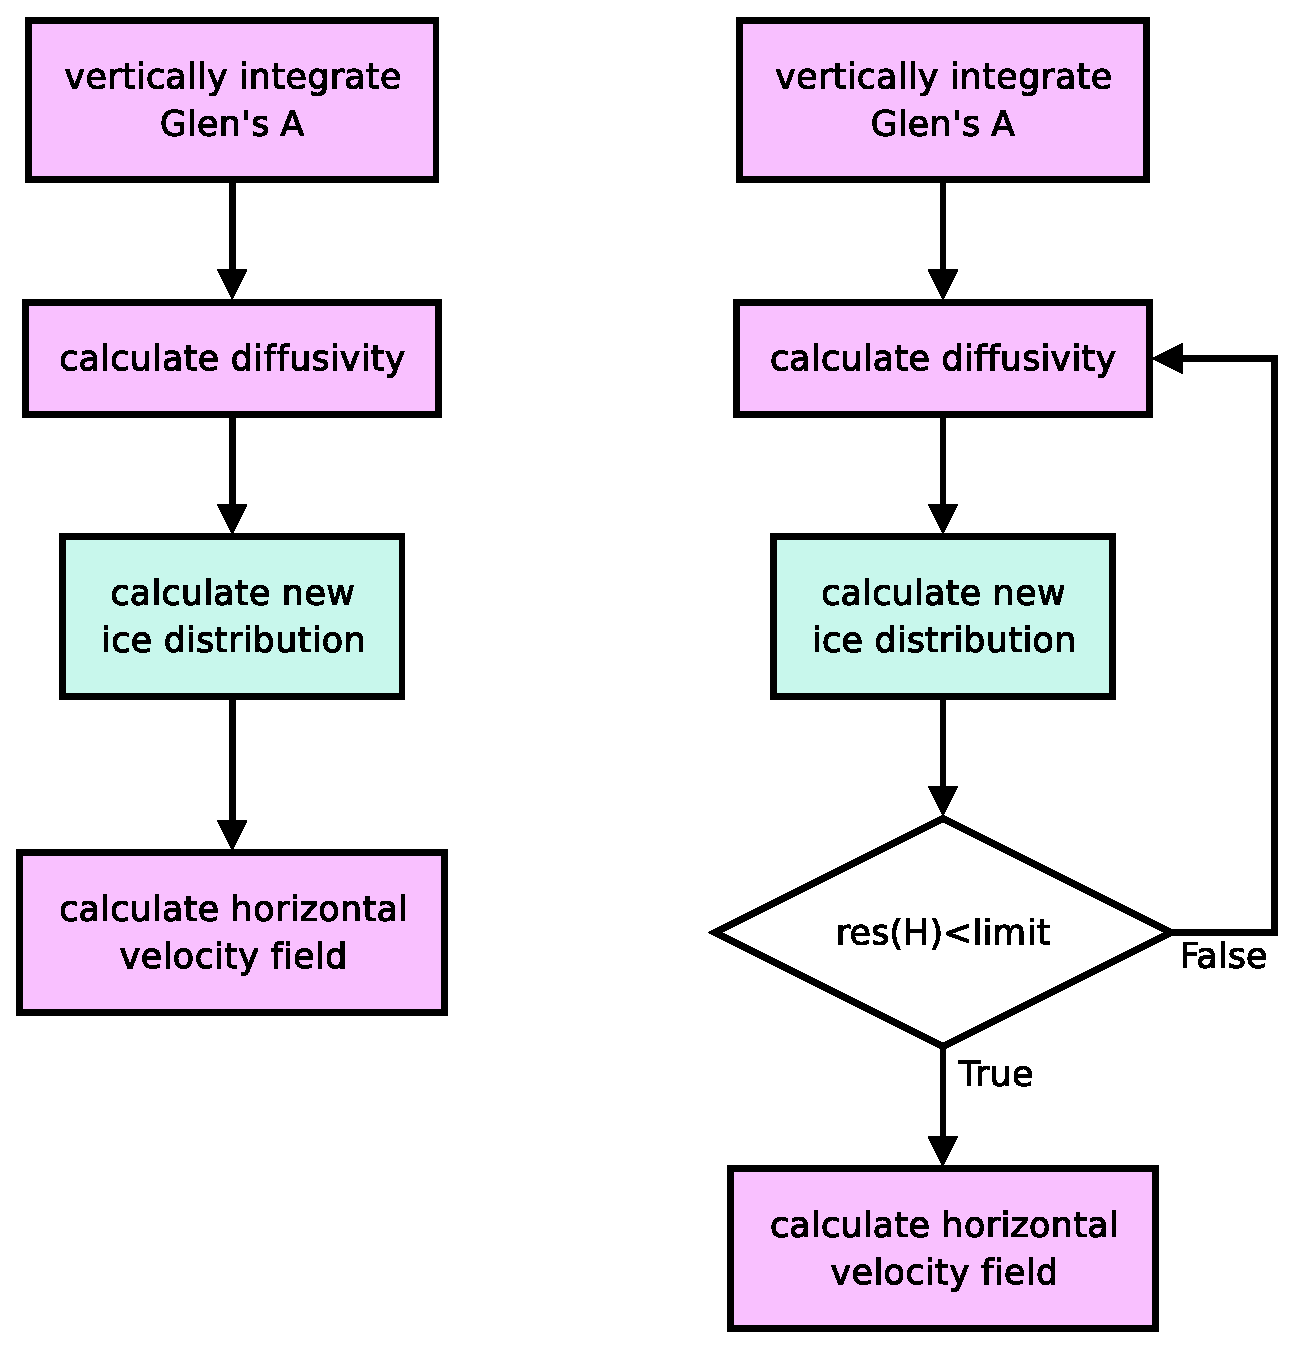
\epsfig{file=\dir/figs/thick_evo.eps,width=0.5\textwidth}
  \caption{Flow diagram showing how the linearised solver (on the left) and the non--linear solver work. The inner, linear iteration is contained within the box labeled ``calculate new ice distribution''.}
  \label{kin.fig.solvers}
\end{figure}

\subsection{Calculating Vertical Velocities}

\subsubsection{Grid Velocity}
The vertical grid moves as a consequence of using a $\sigma$--coordinate system. The grid velocity is
\begin{equation}
  \label{kin.eq.grid_velo}
  w^{\text{grid}}(\sigma)=\frac{\pd s}{\pd t}+\vec u\cdot\vec\nabla s-\sigma\left(\frac{\pd H}{\pd t}+\vec u\cdot\vec\nabla H\right)
\end{equation}
The numerical implementation of Equation \eqref{kin.eq.grid_velo} is straight--forward.

\subsubsection{Vertical Velocity}
The discretised version of the vertical velocity equation \eqref{kin.eq.vert_velo_scaled} is slightly more compilicated because the horizontal velocities are calculated on the $(r,s)$ grid. The vertical velocity at the ice base is $w_{i,j,N}=w^{\text{grid}}_{i,j,N}-b_{i,j}$, where $b_{i,j}$ is the basal melt rate. Integrating from the bottom, the vertical velocity is then
\begin{equation}
  \label{kin.eq.wvel_unc}
  \begin{split}
  w_{i,j,k}=-\sum_{\tilde{k}=N-1}^1\left\{\mathcal{H}_{i,j}\left(\frac{u^x_{i,j,k}+u^x_{i,j,k+1}}{2}+\frac{v^y_{i,j,k}+v^y_{i,j,k+1}}{2}\right)(\sigma_{k+1}-\sigma_k)\right. \\
     +(\tilde{u}_{i,j,k+1}-\tilde{u}_{i,j,k})  \left(\tilde{s}^x_{i,j}-\frac12(\sigma_{k+1}+\sigma_k)\tilde{H}^x_{i,j}\right)  \\
     \left.+(\tilde{v}_{i,j,k+1}-\tilde{v}_{i,j,k})  \left(\tilde{s}^y_{i,j}-\frac12(\sigma_{k+1}+\sigma_k)\tilde{H}^y_{i,j}\right)\right\} + w_{i,j,N}
  \end{split}
\end{equation}
with the weighted ice thickness
\begin{equation*}
  \begin{split}
  \mathcal{H}_{i,j}=\frac{4H_{i,j}+2(H_{i-1,j}+H_{i+1,j}+H_{i,j-1}+H_{i,j+1})}{16}\\
  +\frac{H_{i-1,j-1}+H_{i+1,j-1}+H_{i+1,j+1}+H_{i-1,j+1}}{16}    
  \end{split}
\end{equation*}

This scheme produces vertical velocities at the ice divide which are too small. The vertical velocities on the ice surface are given by the upper kinematic boundary condition, Equation \eqref{kin.eq.upper_bc}. Equation \eqref{kin.eq.wvel_unc} can be corrected with:
\begin{equation}
  \label{kin.eq.wvel_cor}
   w^\ast_{i,j,k}=w_{i,j,k}-(1-\sigma_k)(w_{i,j,k}-{w_s}_{i,j}),
\end{equation}
where ${w_s}_{i,j}$ is the vertical velocity at the ice surface given by \eqref{kin.eq.upper_bc}. Figure \ref{kin.fig.w_profile} shows the different vertical velocities at the ice surface.
\begin{figure}[htbp]
  \centering
  \includegraphics{\dir/gnu/w_profile.eps}
  \caption{Vertical ice surface velocities of the EISMINT-1 moving margin experiment.}
  \label{kin.fig.w_profile}
\end{figure}
The difference between the vertical velocities calculated by the model and the vertical velocities given by \eqref{kin.eq.upper_bc} at the ice margin are due to the fact that temperatures and velocities are only calculated when the ice is thicker than a certain threshold value which is not met at the ice margin.

Figure \ref{kin.fig.wt_sigma} shows vertical profiles of the vertical velocity at the ice divide and a point half--way between the divide and the domain margin. A corresponding temperature profile is also shown since the vertical velocity determines the vertical temperature advection (see Section \ref{temp.sec.vert_ad}).
\begin{figure}[htbp]
  \centering
  \includegraphics{\dir/gnu/wt_sigma.eps}
  \caption{Vertical velocity and temperature distribution for columns at the ice divide and a point half--way between the divide and the domain margin.}
  \label{kin.fig.wt_sigma}
\end{figure}

\section{Temperature Solver}
This document summarises what I have learned by staring at the GLIMMER code and reading various papers.

The ice temperature, $T$, evolves according to
\begin{multline}
  \label{temp.eq.temp}
  \frac{\pd T}{\pd t} = \frac{k}{\rho cH^2}\frac{\pd^2T}{\pd\sigma^2} - \vec{U}\cdot\vec\nabla T + \frac{\sigma g}c\frac{\pd \vec{U}}{\pd\sigma}\cdot\vec\nabla s \\
  + \frac1H\frac{\pd T}{\pd\sigma}\left[w-\frac{\pd s}{\pd t}-\vec{U}\cdot\vec\nabla s+\sigma\left(\frac{\pd H}{\pd t}+\vec{U}\cdot\vec\nabla H\right)\right]
\end{multline}
The terms represents (1) vertical diffusion, (2) horizontal advection, (3) internal heat generation due to friction and (4) vertical advection and a correction due to the sigma coordinate system. Let's rewrite \eqref{temp.eq.temp} to introduce some names:
\begin{equation}
  \label{temp.eq.temp2}
  \frac{\pd T}{\pd t} = a\frac{\pd^2T}{\pd\sigma^2} +b(\sigma) + \Phi(\sigma) + c(\sigma)\frac{\pd T}{\pd\sigma},
\end{equation}
where
\begin{subequations}
  \begin{align}
    a&=\frac{k}{\rho cH^2} \\
    \label{temp.eq.hadv}
    b(\sigma)&=-\vec{U}\cdot\vec\nabla T\\
    \Phi(\sigma)&=\frac{\sigma g}c\frac{\pd \vec{U}}{\pd\sigma}\cdot\vec\nabla s \\
    c(\sigma)&=\frac1H\left[w-\frac{\pd s}{\pd t}-\vec{U}\cdot\vec\nabla s+\sigma\left(\frac{\pd H}{\pd t}+\vec{U}\cdot\vec\nabla H\right)\right]
  \end{align}
\end{subequations}

The horizontal velocity in $x$ direction is given by:
\begin{equation}
  \label{temp.eq.horiz_velo}
  u_x(\sigma) = -2(\rho g)^nH^{n+1}|\vec\nabla s|^{n-1}\frac{\pd s}{\pd x}\int_1^\sigma A(T^\ast)\sigma^nd\sigma+u_x(1)
\end{equation}
The equation for the $y$--velocity, $u_y$ is similar.

\subsection{Vertical Diffusion}
Discretisation of $\pd^2T/\pd\sigma^2$ is slightly complicated because the vertical grid is irregular. Using Taylor series the central difference formulas are
\begin{subequations}
  \begin{align}
    \label{temp.eq.d1}
    \left.\frac{\pd T}{\pd\sigma}\right|_{\sigma_{k-1/2}}&=\frac{T_k-T_{k-1}}{\sigma_k-\sigma_{k-1}}\\
    \intertext{and}
    \label{temp.eq.d2}
    \left.\frac{\pd T}{\pd\sigma}\right|_{\sigma_{k+1/2}}&=\frac{T_{k+1}-T_k}{\sigma_{k+1}-\sigma_k}\\
    \intertext{The second partial derivative is then, also uning central differences:}
    \label{temp.eq.d3}
    \left.\frac{\pd^2 T}{\pd\sigma^2}\right|_{\sigma_k} &= \frac{\left.{\pd T}/{\pd\sigma}\right|_{\sigma_{k+1/2}} - \left.{\pd T}/{\pd\sigma}\right|_{\sigma_{k-1/2}}}{1/2\left(\sigma_{k+1}-\sigma_{k-1}\right)}\\
    \intertext{Inserting \eqref{temp.eq.d1} and \eqref{temp.eq.d2} into \eqref{temp.eq.d3}, we get:}
    \label{temp.eq.d4}
    &=\frac{2(T_{k+1}-T_k)}{(\sigma_{k+1}-\sigma_k)(\sigma_{k+1}-\sigma_{k-1})}-\frac{2(T_k-T_{k-1})}{(\sigma_k-\sigma_{k-1})(\sigma_{k+1}-\sigma_{k-1})}
  \end{align}
\end{subequations}
Finally, the terms of equation \eqref{temp.eq.d4} are rearranged:
\begin{multline}
  \left.\frac{\pd^2 T}{\pd\sigma^2}\right|_{\sigma_k} = \frac{2T_{k-1}}{(\sigma_k-\sigma_{k-1})(\sigma_{k+1}-\sigma_{k-1})} - \frac{2T_k}{(\sigma_{k+1}-\sigma_k)(\sigma_k-\sigma_{k-1})}\\
  + \frac{2T_{k+1}}{(\sigma_{k+1}-\sigma_k)(\sigma_{k+1}-\sigma_{k-1})}
\end{multline}

\subsection{Horizontal Advection}
The horizontal advection term, $- \vec{U}\cdot\vec\nabla T$ is solved using an upwinding scheme. Let's start with the 1--dimensional case. The method discussed can be straightforwadly extented to 2D. As always, the temperature function is expressed as a Taylor series.
\begin{subequations}
  \begin{align}
    \label{temp.eq.taylor1}
    T(x+\Delta x) &=T(x)+\Delta xT'(x)+\frac{\Delta x^2}2T''(x)+\ldots\\
    \intertext{If we subsitute $\Delta x$ with $2\Delta x$, Equation \eqref{temp.eq.taylor1}}
    \label{temp.eq.taylor2}
    T(x+2\Delta x) &=T(x)+2\Delta xT'(x)+2\Delta x^2T''(x)+\ldots
  \end{align}
\end{subequations}
From \eqref{temp.eq.taylor1} and \eqref{temp.eq.taylor2} we can construct a difference formula where the $\mathcal{O}(\Delta x^2)$ error is cancelled, by multiplying \eqref{temp.eq.taylor1} with 4 and substracting the result from \eqref{temp.eq.taylor2}:
\begin{subequations}
  \begin{align}
    \label{temp.eq.forward_h3}
    T_+'(x)&=\frac{4T(x+\Delta x)-T(x+2\Delta x)-3T(x)}{2\Delta x}\\
    \intertext{and similarly for the backward difference:}
    T_-'(x)&=-\frac{4T(x-\Delta x)-T(x-2\Delta x)-3T(x)}{2\Delta x}
    \end{align}
\end{subequations}
So the horizontal advection term in one dimensions becomes:
\begin{equation}
  b_x = -u_x\frac{\pd T}{\pd x}=\frac{-u_x}{2\Delta x}
  \begin{cases}
    -(4T_{i-1}-T_{i-2}-3T_i) & \text{when $u_x>0$} \\
    4T_{i+1}-T_{i+2}-3T_i & \text{when $u_x<0$} \\
  \end{cases}
\end{equation}
A similar expression is found for $b_y$ by simply substituting $y$ for $x$. Finally, the combined horizontal advection term, is simply
\begin{equation}
  b=-\vec{U}\cdot\vec\nabla T=-\left(u_x\frac{\pd T}{\pd x}+u_y\frac{\pd T}{\pd y}\right)=b_x+b_y=b_1+b_2T_i
\end{equation}

\subsection{Heat Generation}
Taking the derivative of \eqref{temp.eq.horiz_velo} with respect to $\sigma$, we get
\begin{equation}
  \frac{\pd u_x}{\pd\sigma} = -2(\rho g)^nH^{n+1}|\vec\nabla s|^{n-1}\frac{\pd s}{\pd x}A(T^\ast)\sigma^n
\end{equation}
Thus,
\begin{equation}
\begin{split}
  \Phi(\sigma) &= \frac{\sigma g}c\frac{\pd \vec{U}}{\pd\sigma}\cdot\vec\nabla s  = \frac{\sigma g}c\left(\frac{\pd u_x}{\pd \sigma}\frac{\pd s}{\pd x} + \frac{\pd u_y}{\pd \sigma}\frac{\pd s}{\pd y}\right)\\
       &= -2(\rho g)^nH^{n+1}|\vec\nabla s|^{n-1}\frac{\sigma g}cA(T^\ast)\sigma^n \left(\left(\frac{\pd s}{\pd x}\right)^2+\left(\frac{\pd s}{\pd y}\right)^2\right) \\
       &= -\frac2{c\rho}(g\sigma\rho)^{n+1}\left(H|\vec\nabla s|\right)^{n+1}A(T^\ast)
\end{split}  
\end{equation}

The constant factor $\frac2{c\rho}(g\sigma\rho)^{n+1}$ is calculated during initialisation in the subroutine \texttt{init\_temp}. This factor is assigned to array \texttt{c1(1:upn)}. \texttt{c1} also includes various scaling factors and the factor $1/16$ to normalise $\bar{A}$.

The next factor, $\left(H|\vec\nabla s|\right)^{n+1}$ is calculated in the subroutine \texttt{finddisp}:
\begin{equation}
  {c_2}_{i,j} = \left(\tilde{H}_{i,j}\sqrt{\tilde{S_x}_{i,j}^2+\tilde{S_y}_{i,j}^2}\right)^{n+1},
\end{equation}
where
\begin{equation}
  \tilde{F}_{i,j}=\frac{F^\ast_{i-1/2,j}+F^\ast_{i+1/2,j}+F^\ast_{i,j-1/2}+F^\ast_{i,j+1/2}}4
\end{equation}
and $F^\ast$ denotes a quantity in the velocity grid.

The final factor is found by averaging over the neighbouring nodes:
\begin{equation}
  \bar{A}_{i,j}=4A_{i,j}+2(A_{i-1,j}+A_{i+1,j}+A_{i,j-1}+A_{i,j+1})+(A_{i-1,j-1}+A_{i+1,j-1}+A_{i+1,j+1}+A_{i-1,j+1})
\end{equation}

\subsection{Vertical Advection}
The vertical advection term, $\pd T/\pd\sigma$ is solved using the central difference formula for unevenly spaced nodes:
\begin{equation}
  \frac{\pd T}{\pd\sigma}=\frac{T_{k+1}-T_{k-1}}{\sigma_{k+1}-\sigma_{k-1}}
\end{equation}

\subsection{Boundary Conditions}
At the upper boundary, ice temperatures are set to the surface temperature, $T_{\text{surf}}$. At the ice base, the boundary condition depends on whether the base is melting or not:
\begin{subequations}
  \begin{align}
    T(1) &= T_{\text{pmp}} \quad\text{if $T(1)\ge T_{\text{pmp}}$}\\
    \left.\frac{\pd T}{\pd\sigma}\right|_{\sigma=1}&=-\frac{GH}k \quad\text{if $T(1)<T_{\text{pmp}}$}\\
    \intertext{If the ice is floating, basal temperatures are kept constant, i.e. }
    \frac{\pd T(1)}{\pd t} & = 0
  \end{align}
\end{subequations}
When the ice is floating, basal temperatures are hold constant.

\subsection{Putting it all together}
Equation \eqref{temp.eq.temp} is solved for each ice column. The horizontal dependency of the horizontal advection term, \eqref{temp.eq.hadv}, is resolved by iterating the vertical solution. Putting the individual terms together using a fully explicit finite differences scheme, Equation \eqref{temp.eq.temp2} becomes
\begin{subequations}
  \begin{multline}
    \label{temp.eq.temp3a}
    \frac{T_{k,t+1}-T_{k,t}}{\Delta t} = \left(\frac{2aT_{k-1,t}}{(\sigma_k-\sigma_{k-1})(\sigma_{k+1}-\sigma_{k-1})} - \frac{2aT_{k,t}}{(\sigma_{k+1}-\sigma_k)(\sigma_k-\sigma_{k-1,t})}\right. \\
    \left.+ \frac{2aT_{k+1,t}}{(\sigma_{k+1}-\sigma_k)(\sigma_{k+1}-\sigma_{k-1})}\right)+{b_1}_{k,t}+{b_2}_kT_{k,t}+\Phi_k+c_k\frac{T_{k+1,t}-T_{k-1,t}}{\sigma_{k+1}-\sigma_{k-1}}
\end{multline}
and similarly the fully implicit scheme
  \begin{multline}
    \label{temp.eq.temp3b}
    \frac{T_{k,t+1}-T_{k,t}}{\Delta t} = \left(\frac{2aT_{k-1,t+1}}{(\sigma_k-\sigma_{k-1})(\sigma_{k+1}-\sigma_{k-1})} - \frac{2aT_{k,t+1}}{(\sigma_{k+1}-\sigma_k)(\sigma_k-\sigma_{k-1,t+1})}\right. \\
    \left.+ \frac{2aT_{k+1,t+1}}{(\sigma_{k+1}-\sigma_k)(\sigma_{k+1}-\sigma_{k-1})}\right)+{b_1}_{k,t+1}+{b_2}_kT_{k,t+1}+\Phi_k+c_k\frac{T_{k+1,t+1}-T_{k-1,t+1}}{\sigma_{k+1}-\sigma_{k-1}}
\end{multline}
\end{subequations}
Taking the average of Equations \eqref{temp.eq.temp3a} and \eqref{temp.eq.temp3b} gives the \emph{Crank--Nicholson scheme}. The resulting equation is then rearranged and terms of $T_{k-1,t+1}$, $T_{k,t+1}$ and $T_{k+1,t+1}$ are combined to give the tri--diagonal system
\begin{equation}
  \alpha_kT_{k-1,t+1}+\beta_kT_{k,t+1}+\gamma_kT_{k+1,t+1}=\delta_k
\end{equation}
where, for $k=2,N-1$
\begin{subequations}
  \begin{align}
    \alpha_k &= -\frac12\frac{2a\Delta t}{(\sigma_k-\sigma_{k-1})(\sigma_{k+1}-\sigma_{k-1})}+\frac12\frac{c_k\Delta t}{\sigma_{k+1}-\sigma_{k-1}} \\
    \beta_k &= 1+\frac12\frac{2a\Delta t}{(\sigma_{k+1}-\sigma_k)(\sigma_k-\sigma_{k-1})}-\frac12{b_2}_k\Delta t=1-\alpha_k-\gamma_k-\frac12{b_2}_k\Delta t\\
    \gamma_k &= -\frac12\frac{2a\Delta t}{(\sigma_{k+1}-\sigma_k)(\sigma_{k+1}-\sigma_{k-1})}-\frac12\frac{c_k\Delta t}{\sigma_{k+1}-\sigma_{k-1}} \\
    \delta_k &= -\alpha_kT_{k-1,t}+(2-\beta_k)T_{k,t}-\gamma_kT_{k+1,t}+\frac12({b_1}_{k,t}+{b_1}_{k,t+1})\Delta t+\Phi_k\Delta t
  \end{align}

\subsubsection{Boundary Conditions}
At the upper boundary:
\begin{equation}
  \alpha_1=0,\quad\beta_1=1,\quad\gamma_1=0,\quad\delta_1=T_{\text{surf}}
\end{equation}
\end{subequations}


The lower boundary condition is somewhat more complicated. Here we only look at the case when the temperature is below the pressure melting point of ice. BC for floating ice and temperatures at the pressure melting point of ice are trivial. The geothermal heat flux is applied at the lower boundary, i.e. Equation \eqref{temp.eq.d2} becomes
\begin{equation}
  \label{temp.eq.d2-lb}
  \left.\frac{\pd T}{\pd\sigma}\right|_{\sigma_{k+1/2}}=-\frac{GH}k
\end{equation}
Assuming that $\sigma_k-\sigma_{k-1}=\sigma_{k+1}-\sigma_k=\Delta\sigma$ and inserting \eqref{temp.eq.d1} and \eqref{temp.eq.d2-lb} into \eqref{temp.eq.d3}, the second partial derivative becomes
\begin{equation}
  \left.\frac{\pd^2 T}{\pd\sigma^2}\right|_{\sigma_N} = \left(-\frac{GH}k-\frac{T_N-T_{N-1}}{\Delta\sigma}\right)/\Delta\sigma=-\frac{GH}{k\Delta\sigma}-\frac{T_N-T_{N-1}}{\Delta\sigma^2}
\end{equation}
Inserting the new conduction term and replacing the derivative of the vertical advection term with the Neuman boundary condition, Equation \eqref{temp.eq.temp3a} becomes
\begin{subequations}
  \begin{equation}
    \frac{T_{N,t+1}-T_{N,t}}{\Delta t} = -a\left(\frac{GH}{k\Delta\sigma}+\frac{T_{N,t}-T_{N-1,t}}{\Delta\sigma^2}\right)+{b_1}_{N,t}+{b_2}_NT_{N,t}+\Phi_N-c_N\frac{GH}k
  \end{equation}
  and similarly for Equation \eqref{temp.eq.temp3b}
  \begin{multline}
    \frac{T_{N,t+1}-T_{N,t}}{\Delta t} = -a\left(\frac{GH}{k\Delta\sigma}+\frac{T_{N,t+1}-T_{N-1,t+1}}{\Delta\sigma^2}\right)+{b_1}_{N,t+1}+{b_2}_NT_{N,t+1}\\
    +\Phi_N-c_N\frac{GH}k
  \end{multline}
\end{subequations}
The elements of the tri--diagonal system at the lower boundary are then
\begin{subequations}
  \begin{gather}
    \alpha_N =-\frac{a\Delta t}{2(\sigma_N-\sigma_{N-1})^2}\\
    \beta_N = 1-\alpha_N+\frac12{b_2}_N\Delta t\\
    \gamma_N = 0 \\
    \begin{split}
      \delta_N =&-\alpha_NT_{N-1,t}+(2-\beta_N)T_{N,t}-a\frac{GH\Delta t}{k(\sigma_N-\sigma_{N-1})}\\
      &+\frac12({b_1}_{N,t}+{b_1}_{N,t+1})\Delta t+\Phi_N\Delta t-c_N\frac{GH\Delta t}k
    \end{split}
  \end{gather}
\end{subequations}


\section{Isostatic Adjustment}
The ice sheet model includes simple approximations for calculating isostatic adjustment. These approximations depend on how the lithosphere and the mantle are treated. For each subsystem there are two models. The lithosphere can be described as a
\begin{description}
\item[\textbf{local lithosphere:}] the flexural rigidity of the lithosphere is ignored, i.e. this is equivalent to ice floating directly on the asthenosphere;
\item[\textbf{elastic lithosphere:}] the flexural rigidity is taken into account;
\end{description}
while the mantle is treated as a
\begin{description}
\item [\textbf{fluid mantle:}] the mantle behaves like a non-viscous fluid, isostatic equilibrium is reached instantaneously;
\item [\textbf{relaxing mantle:}] the flow within the mantle is approximated by an exponentially decaying hydrostatic response function, i.e. the mantle is treated as a viscous half space.
\end{description}

\subsection{Calculation of ice-water load}
At each isostasy time-step, the load of ice and water is calculated, as an
equivalent mantle-depth ($L$). If the basal elevation is above sea-level, then the
load is simply due to the ice:
\begin{equation}
L=\frac{\rho_i}{\rho_m}H,
\label{load_land_ice}
\end{equation}
where $H$ is the ice thickness, with $\rho_i$ and $\rho_m$ being the densities
of the ice and mantle respectively. In the case where the bedrock is below
sea-level, the load is calculated is that due to a change in sea-level rise and/or
the presence of non-floating ice. When the ice is floating ($\rho_i
H<\rho_o(z_0-h)$), the load is only due to sea-level changes
\begin{equation}
L=\frac{\rho_o}{\rho_m}z_0,
\label{load_sea_float}
\end{equation}
whereas when the ice is grounded, it displaces the water, and adds an
additional load:
\begin{equation}
L=\frac{\rho_i H+\rho_o h}{\rho_m}.
\label{load_sea_grounded}
\end{equation}
here, $\rho_o$ is the density of sea water, $z_0$ is the change in sea-level
relative to a reference level and $h$ is the bedrock elevation relative to the
same reference level. The value of $h$ will be negative for submerged bedrock,
hence the plus sign in (\ref{load_sea_grounded}).

\subsection{Elastic lithosphere model}
This is model is selected by setting \texttt{lithosphere = 1} in the
configuration file. By simulatuing the deformation of the lithosphere, the
deformation seen by the aesthenosphere beneath is calculated. In the absence of this
model, the deformation is that due to Archimedes' Principle, as though the
load were floating on the aesthenosphere.

The elastic lithosphere model is based on work by \cite{Lambeck1980}, and its
implementation is fully described in \cite{Hagdorn2003}. The lithosphere
model only affects the geometry of the deformation --- the timescale for
isostatic adjustment is controlled by the aesthenosphere model. 

The load due to a single (rectangular) grid point is approximated as being
applied to a disc of the same area. The deformation due to a disc of ice of
radius $A$ and thickness $H$ is given by these expressions. For $r<A$:
\begin{equation} 
w(r)=\frac{\rho_i H}{\rho_m}\left[1+C_1\,\mathrm{Ber}\left(\frac{r}{L_r}\right)+C_2\,\mathrm{Bei}\left(\frac{r}{L_r}\right)\right],
\end{equation}
and for $r\geq A$:
\begin{equation}
w(r)=\frac{\rho_i
  H}{\rho_m}\left[D_1\,\mathrm{Ber}\left(\frac{r}{L_r}\right)+D_2\,\mathrm{Bei}\left(\frac{r}{L_r}\right)
+D_3\,\mathrm{Ker}\left(\frac{r}{L_r}\right)+D_4\,\mathrm{Kei}\left(\frac{r}{L_r}\right)\right],
\end{equation}
where $\mathrm{Ber}(x)$, $\mathrm{Bei}(x)$, $\mathrm{Ker}(x)$ and
$\mathrm{Kei}(x)$ are Kelvin functions of zero order, $L_r=(D/\rho_m
g))^{1/4}$ is the radius of relative stiffness, and $D$ is the flexural
rigidity. The constants $C_i$ and $D_i$ are given by
\begin{equation}
\begin{array}{rcl}
C_1&=&a\,\mathrm{Ker}'(a)\\
C_2&=&-a\,\mathrm{Ker}'(a)\\
D_1&=&0\\
D_2&=&0\\
D_3&=&a\,\mathrm{Ber}'(a)\\
D_4&=&-a\,\mathrm{Ber}'(a).
\end{array}
\end{equation}
Here, the prime indicates the first spatial derivative of the Kelvin functions.

\subsection{Relaxing aesthenosphere model}
If a fluid mantle is selected, it adjusts instantly to changes in lithospheric
loading. However, a relaxing mantle is also available.

%%% Local Variables: 
%%% mode: latex
%%% TeX-master: "isos"
%%% End: 


\chapter{Developer Guide}
\renewcommand{\dir}{dg}
\newcommand{\dir}{dg}

\pagestyle{myheadings}
\markright{GLIMMER code design overview}

\begin{document}
\title{GLIMMER --- Developer's Guide}
\author{Magnus Hagdorn\thanks{Magnus.Hagdorn@ed.ac.uk} \and Ian Rutt\thanks{I.C.Rutt@bristol.ac.uk}}
\maketitle
\tableofcontents
\newpage

\newcommand{\dir}{dg}

\pagestyle{myheadings}
\markright{GLIMMER code design overview}

\begin{document}
\title{GLIMMER --- Developer's Guide}
\author{Magnus Hagdorn\thanks{Magnus.Hagdorn@ed.ac.uk} \and Ian Rutt\thanks{I.C.Rutt@bristol.ac.uk}}
\maketitle
\tableofcontents
\newpage

\newcommand{\dir}{dg}

\pagestyle{myheadings}
\markright{GLIMMER code design overview}

\begin{document}
\title{GLIMMER --- Developer's Guide}
\author{Magnus Hagdorn\thanks{Magnus.Hagdorn@ed.ac.uk} \and Ian Rutt\thanks{I.C.Rutt@bristol.ac.uk}}
\maketitle
\tableofcontents
\newpage

\input{\dir/dg.tex}
\end{document}
\end{document}
\end{document}

\renewcommand{\dir}{ext}
\newcommand{\dir}{ext}

\pagestyle{myheadings}

\markright{Glimmer-CISM {\glimmerver} Extension documentation}

\begin{document}
\title{Glimmer-CISM {\glimmerver} Extension Documentation}
\author{Magnus Hagdorn\thanks{Magnus.Hagdorn@ed.ac.uk}, Ian
Rutt\thanks{I.C.Rutt@bristol.ac.uk} \and Tony Payne\thanks{a.j.payne@bristol.ac.uk}}

\maketitle
\tableofcontents
\newpage

\newcommand{\dir}{ext}

\pagestyle{myheadings}

\markright{Glimmer-CISM {\glimmerver} Extension documentation}

\begin{document}
\title{Glimmer-CISM {\glimmerver} Extension Documentation}
\author{Magnus Hagdorn\thanks{Magnus.Hagdorn@ed.ac.uk}, Ian
Rutt\thanks{I.C.Rutt@bristol.ac.uk} \and Tony Payne\thanks{a.j.payne@bristol.ac.uk}}

\maketitle
\tableofcontents
\newpage

\newcommand{\dir}{ext}

\pagestyle{myheadings}

\markright{Glimmer-CISM {\glimmerver} Extension documentation}

\begin{document}
\title{Glimmer-CISM {\glimmerver} Extension Documentation}
\author{Magnus Hagdorn\thanks{Magnus.Hagdorn@ed.ac.uk}, Ian
Rutt\thanks{I.C.Rutt@bristol.ac.uk} \and Tony Payne\thanks{a.j.payne@bristol.ac.uk}}

\maketitle
\tableofcontents
\newpage

\input{\dir/ext.tex}
\bibliography{glimmer}
\end{document}

\bibliography{glimmer}
\end{document}

\bibliography{glimmer}
\end{document}


\part{Appendix}
\appendix
\renewcommand{\dir}{ug}
\chapter{netCDF Variables}
%%%%%%%%%%%%%%%%%%%%%%%%%%%%%%%%%%%%%%%%%%%%%%%%%%%%%%%%%%%%%%%%%%%%%%%%%%%%%%%%
% WARNING: this file was automatically generated on
% Tue, 11 Jan 2005 15:56:57 +0000
% from varlist.tex.in
%%%%%%%%%%%%%%%%%%%%%%%%%%%%%%%%%%%%%%%%%%%%%%%%%%%%%%%%%%%%%%%%%%%%%%%%%%%%%%%%

\label{ug.sec.varlist}
The following list shows all the variable names used by GLIMMER. Only variables marked with $^\ast$ are loaded by the input routines. Append \texttt{\_spot} to the variable name to get single location version of the variable.
\begin{center}
    \tablefirsthead{%
    \hline
        Name&  Description & Units\\
    \hline
    \hline}
  \tablehead{%
    \hline
    \multicolumn{3}{|p{0.98\textwidth}|}{\emph{\small continued from previous page}}\\
    \hline
        Name&  Description & Units\\
    \hline
    \hline}
  \tabletail{%
    \hline
    \multicolumn{3}{|r|}{\emph{\small continued on next page}}\\
    \hline}
  \tablelasttail{\hline}
  \begin{supertabular}{|l|p{8cm}|c|}
    \hline
\texttt{ablt} & ablation & meter/year\\
\hline
\texttt{acab} & accumulation, ablation rate & meter/year\\
&CF name: \texttt{land\_ice\_surface\_mass\_balance}&\\
\hline
\texttt{arng} & annual temperature range & degree\_Celcius\\
\hline
\texttt{artm} & annual mean air temperature & degree\_Celcius\\
&CF name: \texttt{surface\_temperature}&\\
\hline
\texttt{bmlt} & basal melt rate & meter/year\\
&CF name: \texttt{land\_ice\_basal\_melt\_rate}&\\
\hline
\texttt{btemp} & basal ice temperature & degree\_Celcius\\
\hline
\texttt{btrc} & basal slip coefficient & meter/pascal/year\\
\hline
\texttt{bwat} & basal water depth & meter\\
\hline
\texttt{diffu} & apparent diffusivity & meter2/year\\
\hline
\texttt{dusrfdtm} & rate of upper ice surface elevation change & meter/year\\
\hline
\texttt{flwa} & ?? & ??\\
\hline
\texttt{lat}$^\ast$ & Latitude & degreeN\\
&CF name: \texttt{latitude}&\\
\hline
\texttt{lon}$^\ast$ & Longitude & degreeE\\
&CF name: \texttt{longitude}&\\
\hline
\texttt{lsurf} & ice lower surface elevation & meter\\
\hline
\texttt{mask}$^\ast$ & upscaling and downscaling mask & 1\\
\hline
\texttt{prcp} & precipitation & meter/year\\
&CF name: \texttt{lwe\_precipitation\_rate}&\\
\hline
\texttt{presprcp}$^\ast$ & present day precipitation & meter/year\\
\hline
\texttt{presusrf}$^\ast$ & present day surface of the ice-sheet & meter\\
\hline
\texttt{relx}$^\ast$ & relaxed bedrock topography & meter\\
\hline
\texttt{std\_dev}$^\ast$ & standard deviation of sub-grid topography & meter\\
\hline
\texttt{temp} & ice temperature & degree\_Celcius\\
&CF name: \texttt{land\_ice\_temperature}&\\
\hline
\texttt{thk} & ice thickness & meter\\
&CF name: \texttt{land\_ice\_thickness}&\\
\hline
\texttt{topg}$^\ast$ & bedrock topography & meter\\
&CF name: \texttt{bedrock\_altitude}&\\
\hline
\texttt{ubas} & basal slip velocity in x direction & meter/year\\
&CF name: \texttt{land\_ice\_basal\_x\_velocity}&\\
\hline
\texttt{uflx} & flux in x direction & meter2/year\\
\hline
\texttt{usurf}$^\ast$ & ice upper surface elevation & meter\\
\hline
\texttt{uvel} & ice velocity in x direction & meter/year\\
&CF name: \texttt{land\_ice\_x\_velocity}&\\
\hline
\texttt{vbas} & basal slip velocity in y direction & meter/year\\
&CF name: \texttt{land\_ice\_basal\_y\_velocity}&\\
\hline
\texttt{vflx} & flux in x direction & meter2/year\\
\hline
\texttt{vvel} & ice velocity in y direction & meter/year\\
&CF name: \texttt{land\_ice\_y\_velocity}&\\
\hline
\texttt{wgrd} & ?? some velo ?? & meter/year\\
\hline
\texttt{wvel} & vertical ice velocity & meter/year\\
&CF name: \texttt{land\_ice\_z\_velocity}&\\
\hline
  \end{supertabular}
\end{center}

\chapter{The GLIMMER API}
\section{GLUM}
GLUM provides some utility subroutines which are shared by all components of GLIMMER.

\subsection{Subroutine \texttt{open\_log}}
\paragraph{Purpose} open and initialise log file

\paragraph{Name and mandatory arguments}
\begin{verbatim}
subroutine open_log
\end{verbatim}

\paragraph{Arguments}
\begin{center}
  \tablefirsthead{%
    \hline
  }
  \tablehead{%
    \hline
    \multicolumn{4}{|p{\textwidth}|}{\emph{\small continued from previous page}}\\
    \hline
  }
  \tabletail{%
    \hline
    \multicolumn{4}{|r|}{\emph{\small continued on next page}}\\
    \hline}
  \tablelasttail{\hline}
  \begin{supertabular*}{\textwidth}{@{\extracolsep{\fill}}lllp{5.5cm}}
    \multicolumn{4}{|l|}{{\bf Mandatory}}\\
    \hline
    \hline
    \multicolumn{4}{|l|}{{\bf Optional}}\\
    \hline
    \texttt{unit} & \texttt{integer} & \texttt{intent(in)} & file unit to use (defualt: 6) \\
    \texttt{fname}& \texttt{character(len=*)} & \texttt{intent(in)} & name of log file (default: \texttt{glide.log})\\ 
  \end{supertabular*}
\end{center}
%%%%%%%%%%%%%%%%%%%%%%%%%%%%%%%%%%%%%%%%%%%%%%%%%%%
\subsection{Subroutine \texttt{ConfigRead}}
\paragraph{Purpose} Read configuration file and store config options.

\paragraph{Name and mandatory arguments}
\begin{verbatim}
subroutine ConfigRead(fname,config)
\end{verbatim}

\paragraph{Arguments}
\begin{center}
  \tablefirsthead{%
    \hline
  }
  \tablehead{%
    \hline
    \multicolumn{4}{|p{\textwidth}|}{\emph{\small continued from previous page}}\\
    \hline
  }
  \tabletail{%
    \hline
    \multicolumn{4}{|r|}{\emph{\small continued on next page}}\\
    \hline}
  \tablelasttail{\hline}
  \begin{supertabular*}{\textwidth}{@{\extracolsep{\fill}}lllp{5.5cm}}
    \multicolumn{4}{|l|}{{\bf Mandatory}}\\
    \hline
    %%
    \texttt{fname} & \texttt{character(len=*)} & \texttt{intent(in)} & name of configuration file to be read\\
    \texttt{config} & \texttt{type(ConfigSection), pointer} & & pointer to first element of linked list containing configuration\\    
  \end{supertabular*}
\end{center}
\paragraph{Additional Notes}
Each section within the configuration file is stored as an element of a linked list. These elements contain another linked list storing the key--value pairs.

%%%%%%%%%%%%%%%%%%%%%%%%%%%%%%%%%%%%%%%%%%%%%%%%%%%
\subsection{Subroutine \texttt{CheckSections}}
\paragraph{Purpose} To check if all sections within a configuration file were subsequently used. Report unused sections to the log.

\paragraph{Name and mandatory arguments}
\begin{verbatim}
subroutine CheckSections(config)
\end{verbatim}
\paragraph{Arguments}
\begin{center}
  \tablefirsthead{%
    \hline
  }
  \tablehead{%
    \hline
    \multicolumn{4}{|p{\textwidth}|}{\emph{\small continued from previous page}}\\
    \hline
  }
  \tabletail{%
    \hline
    \multicolumn{4}{|r|}{\emph{\small continued on next page}}\\
    \hline}
  \tablelasttail{\hline}
  \begin{supertabular*}{\textwidth}{@{\extracolsep{\fill}}lllp{5.5cm}}
    \multicolumn{4}{|l|}{{\bf Mandatory}}\\
    \hline
    %%
    \texttt{config} & \texttt{type(ConfigSection), pointer} & & pointer to first element of linked list containing configuration\\ 
  \end{supertabular*}
\end{center}

%%%%%%%%%%%%%%%%%%%%%%%%%%%%%%%%%%%%%%%%%%%%%%%%%%%
%\subsection{Subroutine \texttt{}}
%\paragraph{Purpose} 
%\paragraph{Name and mandatory arguments}
%\begin{verbatim}
%
%\end{verbatim}
%\paragraph{Arguments}
%\begin{center}
%  \tablefirsthead{%
%    \hline
%  }
%  \tablehead{%
%    \hline
%    \multicolumn{4}{|p{\textwidth}|}{\emph{\small continued from previous page}}\\
%    \hline
%  }
%  \tabletail{%
%    \hline
%    \multicolumn{4}{|r|}{\emph{\small continued on next page}}\\
%    \hline}
%  \tablelasttail{\hline}
%  \begin{supertabular*}{\textwidth}{@{\extracolsep{\fill}}lllp{5.5cm}}
%    \multicolumn{4}{|l|}{{\bf Mandatory}}\\
%    \hline
%    %%
%    \hline
%    \multicolumn{4}{|l|}{{\bf Optional}}\\
%    \hline
%    %%
%  \end{supertabular*}
%\end{center}


\section{GLIDE}\label{ug.sec.glide_api}
%%%%%%%%%%%%%%%%%%%%%%%%%%%%%%%%%%%%%%%%%%%%%%%%%%
\subsection{Subroutine \texttt{glide\_initialise}}
\paragraph{Purpose} To initialise the basic ice sheet model
\paragraph{Name and mandatory arguments}
\begin{verbatim}
subroutine glide_initialise(model,config)
\end{verbatim}
\paragraph{Arguments}
\begin{center}
  \tablefirsthead{%
    \hline
  }
  \tablehead{%
    \hline
    \multicolumn{4}{|p{0.98\textwidth}|}{\emph{\small continued from previous page}}\\
    \hline
  }
  \tabletail{%
    \hline
    \multicolumn{4}{|r|}{\emph{\small continued on next page}}\\
    \hline}
  \tablelasttail{\hline}
  \begin{supertabular}{lllp{5.5cm}}
    \multicolumn{4}{|l|}{{\bf Mandatory}}\\
    \hline
    %%
    \texttt{model} & \texttt{type(glide\_global\_type)} &\texttt{intent(inout)}& f95 type containing all variables associated with an instance of the model.\\
    \texttt{config} & \texttt{type(ConfigSection), pointer} & & pointer to first element of linked list containing configuration\\ 
  \end{supertabular}
\end{center}
\paragraph{Additional Notes}
This subroutine initialises the model. Memory for all variables is allocated. Input files are opend and read. Output files are created. Variables are scaled.

%%%%%%%%%%%%%%%%%%%%%%%%%%%%%%%%%%%%%%%%%%%%%%%%%%%
\subsection{Subroutine \texttt{glide\_nc\_fillall}}
\paragraph{Purpose} fill netCDF coordinate variables.
\paragraph{Name and mandatory arguments}
\begin{verbatim}
subroutine glide_nc_fillall(model)
\end{verbatim}
\paragraph{Arguments}
\begin{center}
  \tablefirsthead{%
    \hline
  }
  \tablehead{%
    \hline
    \multicolumn{4}{|p{0.98\textwidth}|}{\emph{\small continued from previous page}}\\
    \hline
  }
  \tabletail{%
    \hline
    \multicolumn{4}{|r|}{\emph{\small continued on next page}}\\
    \hline}
  \tablelasttail{\hline}
  \begin{supertabular}{lllp{5.5cm}}
    \multicolumn{4}{|l|}{{\bf Mandatory}}\\
    \hline
    %%
    \texttt{model} & \texttt{type(glide\_global\_type)} &\texttt{intent(inout)}& f95 type containing all variables associated with an instance of the model.\\
  \end{supertabular}
\end{center}

%%%%%%%%%%%%%%%%%%%%%%%%%%%%%%%%%%%%%%%%%%%%%%%%%%%
\subsection{Subroutine \texttt{glide\_tstep\_p1}}
\paragraph{Purpose} Performs first part of time-step of an ice model instance: calculate vertical velocity and temperature field. Set model time.
\paragraph{Name and mandatory arguments}
\begin{verbatim}
subroutine glide_tstep_p1(model,time)
\end{verbatim}
\paragraph{Arguments}
\begin{center}
  \tablefirsthead{%
    \hline
  }
  \tablehead{%
    \hline
    \multicolumn{4}{|p{0.98\textwidth}|}{\emph{\small continued from previous page}}\\
    \hline
  }
  \tabletail{%
    \hline
    \multicolumn{4}{|r|}{\emph{\small continued on next page}}\\
    \hline}
  \tablelasttail{\hline}
  \begin{supertabular}{lllp{5.5cm}}
    \multicolumn{4}{|l|}{{\bf Mandatory}}\\
    \hline
    %%
    \texttt{model} & \texttt{type(glide\_global\_type)} &\texttt{intent(inout)}& f95 type containing all variables associated with an instance of the model.\\
    \texttt{time}  & \texttt{real(rk)} & \texttt{intent(in)} & Current time in years\\
  \end{supertabular}
\end{center}


%%%%%%%%%%%%%%%%%%%%%%%%%%%%%%%%%%%%%%%%%%%%%%%%%%%
\subsection{Subroutine \texttt{glide\_tstep\_p2}}
\paragraph{Purpose} Performs second part of time-step of an ice model instance: write data and move ice and update horizontal velocities.
\paragraph{Name and mandatory arguments}
\begin{verbatim}
subroutine glide_tstep_p2(model)
\end{verbatim}
\paragraph{Arguments}
\begin{center}
  \tablefirsthead{%
    \hline
  }
  \tablehead{%
    \hline
    \multicolumn{4}{|p{0.98\textwidth}|}{\emph{\small continued from previous page}}\\
    \hline
  }
  \tabletail{%
    \hline
    \multicolumn{4}{|r|}{\emph{\small continued on next page}}\\
    \hline}
  \tablelasttail{\hline}
  \begin{supertabular}{lllp{5.5cm}}
    \multicolumn{4}{|l|}{{\bf Mandatory}}\\
    \hline
    %%
    \texttt{model} & \texttt{type(glide\_global\_type)} &\texttt{intent(inout)}& f95 type containing all variables associated with an instance of the model.\\
  \end{supertabular}
\end{center}

%%%%%%%%%%%%%%%%%%%%%%%%%%%%%%%%%%%%%%%%%%%%%%%%%%%
\subsection{Subroutine \texttt{glide\_tstep\_p3}}
\paragraph{Purpose} Performs third part of time-step of an ice model instance: calculate isostatic adjustment and upper and lower ice surface.
\paragraph{Name and mandatory arguments}
\begin{verbatim}
subroutine glide_tstep_p3(model)
\end{verbatim}
\paragraph{Arguments}
\begin{center}
  \tablefirsthead{%
    \hline
  }
  \tablehead{%
    \hline
    \multicolumn{4}{|p{0.98\textwidth}|}{\emph{\small continued from previous page}}\\
    \hline
  }
  \tabletail{%
    \hline
    \multicolumn{4}{|r|}{\emph{\small continued on next page}}\\
    \hline}
  \tablelasttail{\hline}
  \begin{supertabular}{lllp{5.5cm}}
    \multicolumn{4}{|l|}{{\bf Mandatory}}\\
    \hline
    %%
    \texttt{model} & \texttt{type(glide\_global\_type)} &\texttt{intent(inout)}& f95 type containing all variables associated with an instance of the model.\\
  \end{supertabular}
\end{center}

%%%%%%%%%%%%%%%%%%%%%%%%%%%%%%%%%%%%%%%%%%%%%%%%%%%
\subsection{Subroutine \texttt{glide\_finalise}}
\paragraph{Purpose} To shut--down model, close all open files and deallocate memory.
\paragraph{Name and mandatory arguments}
\begin{verbatim}
subroutine glide_finalise(model)
\end{verbatim}
\paragraph{Arguments}
\begin{center}
  \tablefirsthead{%
    \hline
  }
  \tablehead{%
    \hline
    \multicolumn{4}{|p{0.98\textwidth}|}{\emph{\small continued from previous page}}\\
    \hline
  }
  \tabletail{%
    \hline
    \multicolumn{4}{|r|}{\emph{\small continued on next page}}\\
    \hline}
  \tablelasttail{\hline}
  \begin{supertabular}{lllp{5.5cm}}
    \multicolumn{4}{|l|}{{\bf Mandatory}}\\
    \hline
    %%
    \texttt{model} & \texttt{type(glide\_global\_type)} &\texttt{intent(inout)}& f95 type containing all variables associated with an instance of the model.\\
    \hline
    \multicolumn{4}{|l|}{{\bf Optional}}\\
    \hline
    %%
    \texttt{crash} & \texttt{logical} & \texttt{intent(in)} & set to true if the model died unexpectedly \\
  \end{supertabular}
\end{center}


%%%%%%%%%%%%%%%%%%%%%%%%%%%%%%%%%%%%%%%%%%%%%%%%%%%
%\subsection{Subroutine \texttt{}}
%\paragraph{Purpose} 
%\paragraph{Name and mandatory arguments}
%\begin{verbatim}
%
%\end{verbatim}
%\paragraph{Arguments}
%\begin{center}
%  \tablefirsthead{%
%    \hline
%  }
%  \tablehead{%
%    \hline
%    \multicolumn{4}{|p{0.98\textwidth}|}{\emph{\small continued from previous page}}\\
%    \hline
%  }
%  \tabletail{%
%    \hline
%    \multicolumn{4}{|r|}{\emph{\small continued on next page}}\\
%    \hline}
%  \tablelasttail{\hline}
%  \begin{supertabular}{lllp{5.5cm}}
%    \multicolumn{4}{|l|}{{\bf Mandatory}}\\
%    \hline
%    %%
%    \hline
%    \multicolumn{4}{|l|}{{\bf Optional}}\\
%    \hline
%    %%
%  \end{supertabular}
%\end{center}


%
\section{GLINT}
This appendix details the subroutine calls provided by GLINT, and their
arguments. Note that where a type is given as \texttt{real(rk)}, this
indicates that the kind of the real type is specified by the value of
the parameter \texttt{rk}, which may be altered at compile-time (see appropriate
other documentation for details).
%
%%%%%%%%%%%%%%%%%%%%%%%%%%%%%%%%%%%%%%%%%%%%%%%
% INITIALISE_GLINT                            %
%%%%%%%%%%%%%%%%%%%%%%%%%%%%%%%%%%%%%%%%%%%%%%%
%
\subsection{Subroutine \texttt{initialise\_glint}}
%
\paragraph{Purpose} To initialise the ice model, and load in all relevant parameter files.
%
\paragraph{Name and mandatory arguments}
%
\begin{verbatim}
  subroutine initialise_glint(params,lats,longs,paramfile)
\end{verbatim}
%
\paragraph{Arguments}
%
\begin{center}
  \tablefirsthead{%
    \hline
  }
  \tablehead{%
    \hline
    \multicolumn{4}{|p{\textwidth}|}{\emph{\small continued from previous page}}\\
    \hline
  }
  \tabletail{%
    \hline
    \multicolumn{4}{|r|}{\emph{\small continued on next page}}\\
    \hline}
  \tablelasttail{\hline}
  \begin{supertabular*}{\textwidth}{@{\extracolsep{\fill}}lllp{5.5cm}}
    \multicolumn{4}{|l|}{{\bf Mandatory}}\\
    \hline
    \texttt{params}    & \texttt{type(glint\_params)} & \texttt{intent(inout)} &
    Ice model to be configured \\
    \texttt{lats(:)}   & \texttt{real(rk)} & \texttt{intent(in)} & latitudinal
    location of grid-points in global data (given in $^{\circ}\mathrm{N}$)\\ 
    \texttt{longs(:)}  & \texttt{real(rk)} & \texttt{intent(in)} & longitudinal
    location of grid-points in global data (given in $^{\circ}\mathrm{E}$)\\ 
    \texttt{paramfile} & \texttt{character(*)} & \texttt{intent(in)} & name of
    top-level parameter file \\
    \hline
    \multicolumn{4}{|l|}{{\bf Optional}}\\
    \hline
    \texttt{latb(:)} & \texttt{real(rk)} & \texttt{intent(in)} & Latiudinal
    locations of grid-box boundaries (degrees). This array has one more
    element than \texttt{lats}. \\ 
    \texttt{lonb(:)} & \texttt{real(rk)} & \texttt{intent(in)} & Longitudinal
    locations of grid-box boundaries (degrees). This array has one more
    element than \texttt{longs}. \\
    \texttt{orog(:,:)} & \texttt{real(rk)} & \texttt{intent(out)} & The
    initial orography (m). \\
    \texttt{albedo} & \texttt{real(rk)} & \texttt{intent(out)} & The initial
    ice albedo field \\
    \texttt{ice\_frac} & \texttt{real(rk)} & \texttt{intent(out)} & The initial
    ice fraction \\
    \texttt{orog\_lats} & \texttt{real(rk)} & \texttt{intent(in)} &
    Latitudinal location of gridpoints for global orography output\\
    \texttt{orog\_longs} & \texttt{real(rk)} & \texttt{intent(in)} &
    Longitudinal location of gridpoints for global orography output\\
    \texttt{orog\_latb} & \texttt{real(rk)} & \texttt{intent(in)} & Locations
    of the latitudinal boundaries of the grid-boxes (orography)\\
    \texttt{orog\_lonb} & \texttt{real(rk)} & \texttt{intent(in)} & Locations
    of the longitudinal boundaries of the grid-boxes (orography)\\
    \texttt{output\_flag} & \texttt{logical} & \texttt{intent(out)} & Set to
    show outputs have been updated (provided for consistency with main
    \texttt{glint} subroutine).\\
  \end{supertabular*}
\end{center}
%
\paragraph{Additional notes}
%
\begin{itemize}
\item The ice model determines the size of the global domain from the sizes of
  the arrays \texttt{lats} and \texttt{longs}.
\item The latitudes contained in \texttt{lats} must be in descending order, so
  that $\mathtt{lats(i)}>\mathtt{lats(i+1)}$ for $1\leq \mathtt{i} \leq
  \mathtt{size(lats)}$.
\item The optional arguments \texttt{orog\_lats}, \texttt{orog\_longs},
  \texttt{orog\_latb}, and \texttt{orog\_lonb} may be used to define the frid
  on which the orography is output from GLINT. This is useful if the global
  model has spectral dynamics, and thus a higher-resolution orography is
  needed for greater accuracy when transforming to spectral space. These
  arguments may not be present in arbitrary combinations - only
  \texttt{orog\_lats}+\texttt{orog\_longs},
  \texttt{orog\_lats}+\texttt{orog\_longs}+\texttt{orog\_latb},
  \texttt{orog\_lats}+\texttt{orog\_longs}+\texttt{orog\_lonb}, and
  \texttt{orog\_lats}+\texttt{orog\_longs}+\texttt{orog\_latb}+\texttt{orog\_lonb}
  are permitted. Other combinations will generate a fatal error.
\end{itemize}
%
%%%%%%%%%%%%%%%%%%%%%%%%%%%%%%%%%%%%%%%%%%%%%%%
% GLINT                                       %
%%%%%%%%%%%%%%%%%%%%%%%%%%%%%%%%%%%%%%%%%%%%%%%
%
\subsection{Subroutine \texttt{glint}}
%
\paragraph{Purpose}
%
To perform temporal averaging of input fields, and, if necessary, down-scale
those fields onto local projections and perform an ice model time-step. Output
files may be appended to, and if optional arguments used, fields made
available for feedback.
%
\paragraph{Name and mandatory arguments}
%
\begin{verbatim}
  subroutine glint(params,time,temp,precip,zonwind,merwind,orog)
\end{verbatim}
%
\paragraph{Arguments}
%
\begin{center}
  \tablefirsthead{%
    \hline
  }
  \tablehead{%
    \hline
    \multicolumn{4}{|p{\textwidth}|}{\emph{\small continued from previous page}}\\
    \hline
  }
  \tabletail{%
    \hline
    \multicolumn{4}{|r|}{\emph{\small continued on next page}}\\
    \hline}
  \tablelasttail{\hline}
  \begin{supertabular*}{\textwidth}{@{\extracolsep{\fill}}lllp{5.5cm}}
    \multicolumn{4}{|l|}{{\bf Mandatory}}\\
    \hline
    \texttt{params} & \texttt{type(glint\_params)} & \texttt{intent(inout)} &
    parameters for this run \\
    \texttt{time} & \texttt{integer} & \texttt{intent(in)} & Current model time
    (hours) \\
    \texttt{temp(:,:)} & \texttt{real(rk)} & \texttt{intent(in)} & Surface
    temperature field ($^{\circ}\mathrm{C}$) \\
    \texttt{precip(:,:)} & \texttt{real(rk)} & \texttt{intent(in)} & Precipitation field (mm/s) \\
    \texttt{zonwind(:,:)} & \texttt{real(rk)} & \texttt{intent(in)} & Zonal
    component of the wind field ($\mathrm{ms}^{-1}$) \\
    \texttt{merwind(:,:)} & \texttt{real(rk)} & \texttt{intent(in)} & Meridional 
    component of the wind field ($\mathrm{ms}^{-1}$) \\
    \texttt{orog(:,:)} & \texttt{real(rk)} & \texttt{intent(in)} & Global orography (m) \\
    \hline
    \multicolumn{4}{|l|}{{\bf Optional}}\\
    \hline
    \texttt{output\_flag} & \texttt{logical} & \texttt{intent(out)} & Set to show
    new output fields have been calculated after an ice-model time-step. If this
    flag is not set, the output fields retain their values at input. \\ 
    \texttt{orog\_out(:,:)} & \texttt{real(rk)} & \texttt{intent(inout)} & Output
    orography (m)\\ 
    \texttt{albedo(:,:)} & \texttt{real(rk)} & \texttt{intent(inout)} & Surface
    albedo \\
    \texttt{ice\_frac(:,:)} & \texttt{real(rk)} & \texttt{intent(inout)} &
    Fractional ice coverage \\
    \texttt{water\_in(:,:)} & \texttt{real(rk)} & \texttt{intent(inout)} & The
    input fresh-water flux (mm, over ice time-step). Essentially precip, but
    provided for consistency.\\
    \texttt{water\_out(:,:)} & \texttt{real(rk)} & \texttt{intent(inout)} & The
    output fresh-water flux (mm, over ice time-step). This is simply the ablation calculated by
    the model, scaled up to the global grid. It is up to the global model to
    then  deal with it (route it to the oceans, land scheme, etc.) Note that
    the precipitation fed to the model but which doesn't get incorporated into
    the ice sheet because it falls over the sea is returned in this field. \\ 
    \texttt{total\_water\_in} & \texttt{real(rk)} & \texttt{intent(inout)} &
    Area-integrated water flux in (kg)\\ 
    \texttt{total\_water\_out} & \texttt{real(rk)} & \texttt{intent(inout)} &
    Area-integrated water flux out (kg)\\
    \texttt{ice\_volume} & \texttt{real(rk)} & \texttt{intent(inout)} & Total ice volume (m$^3$)\\
  \end{supertabular*}
\end{center}
\paragraph{Additional notes}
%
\begin{itemize}
\item The sizes of all two-dimensional fields passed as arguments must be the
  same as that implied by the sizes of the arrays used to pass latitude and
  longitude information when the model was initialised using
  \texttt{initialise\_glint}. There is
  currently no checking mechanism in place for this, so using fields of the wrong size
  will lead to unpredictable results.
\item Zonal and meridional components of the wind are only required if the
  small-scale precipitation parameterization is being used (with
  \texttt{whichprecip} set to 2). In other circumstances, \texttt{zonwind} and
  \texttt{merwind} must still be arrays of the correct rank, but need not be
  the correct size, or may be unallocated if desired (this should be changed
  at some point).
\item The output field arguments only return data relevant to the parts of the globe
  covered by the ice model instances. The fraction of each global
  grid-box covered by ice model instances may be obtained using the
  \texttt{glint\_coverage\_map} subroutine below. 
\item The output orography field is given as a mean calculated over the part
  of the grid-box covered by ice  model instances. Thus, to calculate the
  grid-box mean, the output fields should be multiplied point-wise by the
  coverage fraction. 
\item Albedo is currently fixed at 0.4 for ice-covered ground, and set to zero
  elsewhere. The albedo is given for the part of the global grid box covered
  by ice, not as an average of the part covered by the ice model. No attempt
  is made to guess the albedo of the parts of the ice model domain \emph{not}
  covered by ice.
\end{itemize}
%
\paragraph{Example interpretation of output fields}
%
Consider a particular point, $(i,j)$ in the global domain. Suppose value
returned by \texttt{glint\_coverage\_map} for this point is 0.7, and the
output fields have these values:
\begin{verbatim}
  orog_out(i,j)  = 200.0
  albedo(i,j)    =   0.4
  ice_frac(i,j)  =   0.5
\end{verbatim}
%
What does this mean? Well, the ice model covers 70\% of the grid-box, and in
that part the mean surface elevation is 200\,m. Of the part covered by the ice
model, half is actually covered by ice. Thus, 35\% ($0.5\times 0.7$) of the global grid-box is
covered by ice, and the ice has an mean albedo of 40\%. The model makes no suggestion for the
albedo or elevation of the other 65\% of the grid-box. Currently, ice albedo
is a constant that may be changed in the appropriate configuration file, but
this output field is provided against the possibility that the model may be
extended at some point to include a model of ice albedo.
%
%%%%%%%%%%%%%%%%%%%%%%%%%%%%%%%%%%%%%%%%%%%%%%%
% END_GLINT                                   %
%%%%%%%%%%%%%%%%%%%%%%%%%%%%%%%%%%%%%%%%%%%%%%%
%
\subsection{Subroutine \texttt{end\_glint}}
%
\paragraph{Purpose} To perform general tidying-up operations, close files, etc.
%
\paragraph{Name and mandatory arguments}
%
\begin{verbatim}
  subroutine end_glint(params)
\end{verbatim}
%
\paragraph{Arguments}
%
\begin{center}
  \tablefirsthead{%
    \hline
  } 
  \tablehead{%
    \hline
    \multicolumn{4}{|p{\textwidth}|}{\emph{\small continued from previous page}}\\
    \hline
  } 
  \tabletail{%
    \hline
    \multicolumn{4}{|r|}{\emph{\small continued on next page}}\\
    \hline}
      \tablelasttail{\hline}
        \begin{supertabular*}{\textwidth}{@{\extracolsep{\fill}}lllp{5.5cm}}
          \texttt{params} & \texttt{type(glint\_params)} & \texttt{intent(inout)} & Ice model paramters \\
\end{supertabular*}
\end{center}
%
%%%%%%%%%%%%%%%%%%%%%%%%%%%%%%%%%%%%%%%%%%%%%%%
% GLINT_COVERAGE_MAP                          %
%%%%%%%%%%%%%%%%%%%%%%%%%%%%%%%%%%%%%%%%%%%%%%%
%
\subsection{Function \texttt{glint\_coverage\_map}}
%
\paragraph{Purpose} To obtain a map of fractional coverage of global
grid-boxes by the ice model instances. The function returns a value
indicating success, or giving error information.
%
\paragraph{Type, name and mandatory arguments}
%
\begin{verbatim}
  integer function glint_coverage_map(params,coverage,cov_orog)
\end{verbatim}
%
\paragraph{Arguments}
%
\begin{center}
  \tablefirsthead{%
    \hline
  } 
  \tablehead{%
    \hline
    \multicolumn{4}{|p{\textwidth}|}{\emph{\small continued from previous page}}\\
    \hline
  } 
  \tabletail{%
    \hline
    \multicolumn{4}{|r|}{\emph{\small continued on next page}}\\
    \hline}
      \tablelasttail{\hline}
        \begin{supertabular*}{\textwidth}{@{\extracolsep{\fill}}lllp{5.5cm}}
        \texttt{params} & \texttt{type(glint\_params)} & \texttt{intent(in)} & Ice model parameters \\
\texttt{coverage(:,:)} & \texttt{real(rk)} & \texttt{intent(out)} & Coverage
map (all fields except orography) \\
\texttt{cov\_orog(:,:)} & \texttt{real(rk)} & \texttt{intent(out)} & Coverage
map (orography) \\
\end{supertabular*}
\end{center}
%
\paragraph{Returned value}
%
\begin{center}
\begin{tabular}{cl}
\hline
Value & Meaning \\
\hline
\hline
0 & Coverage maps have been returned successfully \\
1 & Coverage maps not yet calculated; must call \texttt{initialise\_glint}
first \\
2 & Arrays \texttt{coverage} or \texttt{cov\_orog} are the wrong size \\
\hline
\end{tabular}
\end{center}

\renewcommand{\dir}{ext}
\input{\dir/selected_ext.tex}

\let\olddir\dir

\ifthenelse{\boolean{have_libphaml}} {
      \renewcommand{\dir}{\olddir/libphaml}
      

%code framing environment-------------------------------
%parameter 1 is code to be framed
%displays code framed in a box, single spaced, normal font
\newenvironment{framecode}[1]%
{
 \vspace{.5cm} 
 \begin{center}
 \begin{Sbox}
 \begin{minipage}{#1}

}
{
 \end{minipage}
 \end{Sbox}
 \fbox{\TheSbox}
 \end{center}
 }


%------------------------------------------------------

\newcommand{\appdir}{}

\newenvironment{dispcode}[3]%
{
\section{#1}\label{#3}
\begin{footnotesize}
\verbatiminput{\appdir/#2}
\end{footnotesize}
}
{

}



\chapter{Libphaml}

\section{SETUP}\label{ch:setup}
%%%%%%%%%%%%%%%%%%%%%%%%%%%%%%%%%%%%%%%%%%%%%%%%%%%%%%%%%%%%%%%%%%%%%%%%%%%%%%%%
\section{Introduction}
This appendix presents some compilation notes for the Fortran source files, these can be found in the \href{http://developer.berlios.de/projects/glimmer-cism/}{Glimmer-CISM2} project on the Berlios SVN server.  These include the following files:
\href{http://svn.berlios.de/svnroot/repos/glimmer-cism/glimmer-cism2/libphaml/phaml\_user\_mod.F90}{phaml\_user\_mod.F90},
\href{http://svn.berlios.de/svnroot/repos/glimmer-cism/glimmer-cism2/libphaml/phaml\_support.F90}{phaml\_support.F90},
\href{http://svn.berlios.de/svnroot/repos/glimmer-cism/glimmer-cism2/libphaml/phaml\_pde.F90}{phaml\_pde.F90},
\href{http://svn.berlios.de/svnroot/repos/glimmer-cism/glimmer-cism2/libphaml/phaml\_example.F90}{phaml\_example.F90},
\href{http://svn.berlios.de/svnroot/repos/glimmer-cism/glimmer-cism2/libphaml/phaml\_example\_pde.F90}{phaml\_example\_pde.F90}, and 
\href{http://svn.berlios.de/svnroot/repos/glimmer-cism/glimmer-cism2/libphaml/simple\_phaml.F90}{simple\_phaml.F90}.

These instructions all assume a POSIX-compatible system.  Although all of the software can be compiled on other operating systems, this has not been attempted on any other OS and therefore is absent.  PHAML must be compiled after the graphics libraries if the OpenGL graphics are desired.  The graphic libraries are optional though and unnecessary for running the ice sheet model.  They are merely present for extra visual output if desired.


All projects require make to build.  For the following instructions, the assumption will be made that a global programs directory exists at /usr/bin.  If the target system does not have this, then it is necessary to register the installation directory with the system globally so that other programs can find it.
%%%%%%%%%%%%%%%%%%%%%%%%%%%%%%%%%%%%%%%%%%%%%%%%%%%%%%%%%%%%%%%%%%%%%%%%%%%%%%%%
\section{Triangle}
\subsection{Compiling/Installing}
Triangle must be compiled separate from PHAML and installed.  This process is straightforward.  A program called showme is also compiled and can be installed.  It allows you to view the mesh files that Triangle generates which is useful for testing purposes.

\begin{framecode}{6in}
\begin{verbatim}

make
cp triangle /usr/bin
cp showme /usr/bin

\end{verbatim}
\end{framecode}

%%%%%%%%%%%%%%%%%%%%%%%%%%%%%%%%%%%%%%%%%%%%%%%%%%%%%%%%%%%%%%%%%%%%%%%%%%%%%%%%
\section{PHAML}

\subsection{Getting PHAML}
PHAML can be downloaded as an archive from the website \cite{PHAML:website}, and then unarchived into a directory anywhere on the system.

\subsection{Compiling PHAML}

PHAML is relatively easy to compile if all the library dependencies are satisfied.  The list of dependencies as well as instructions for additional libraries are at the end of this section.  The PHAML user guide \cite{phamldoc} has an excellent section covering setting up some of these libraries and dependencies as well.  The Quickstart guide is a must read before attempting any serious PHAML work.  A lot more detail is also provided on individual software packages that can be used and the benefits they can provide.  These instructions will now assume that the minimum requirements are met.

First the document `mkmkfile.sh' needs to be edited in the root directory of the PHAML source folder.  The following items must be set correctly: DEFAULT\_PHAML\_ARCH, \\ DEFAULT\_PHAML\_OS, DEFAULT\_PHAML\_F90, DEFAULT\_PHAML\_C, \\ DEFAULT\_PHAML\_PARLIB, DEFAULT\_PHAML\_BLAS, and DEFAULT\_PHAML\_LAPACK.  
All other variables can be left to their default value.  The file `mkmkfile.sh' lists the available options for each of these as well.  A brief overview of these are in the dependencies section below.  Once these variables have all been correctly set the file can be closed and run as a script.  As the name suggests, this scripts generates the makefile needed to compile the project with make.

Now just invoke make and it should compile provided things were set correctly.

\begin{framecode}{6in}
\begin{verbatim}

./mkmkfile.sh
make

\end{verbatim}
\end{framecode}

If the code does not compile then either the configuration file is incorrect or a dependency is unsatisfied.


\subsubsection{PHAML Dependencies}
These are required dependencies in order to compile and use PHAML.  
\begin{itemize}
    \item \textbf{POSIX compliance} - An operating system must be Unix compatible in order to properly work with PHAML.  Ubuntu was used for all test work.
    \item \textbf{Make} - The compile system. 
    \item \textbf{A Fortran Compiler} - Most Fortran compilers will work.  GFortran was the compiler it was tested against.
    \item \textbf{A C Compiler} - CC or GCC.  GCC was used.
    \item \textbf{MPI Library} - An MPI server must be running in order for PHAML to communicate with its subprocesses.  Openmpi was chosen for all tests.
    \item \textbf{BLAS} - Compiled from source.
    \item \textbf{LAPACK} - Compiled from source.
    \item \textbf{TRIANGLE} - Compiled from source.  Instructions are above.
\end{itemize}
 

\subsubsection{PHAML Additional Libraries}
PHAML covers all additional libraries in the user guide.  The only extra libraries used in this project were the graphic libraries which have a separate section below with instructions.
\begin{itemize}
    \item \textbf{OpenGL} - The main graphics library.
    \item \textbf{GLUT} - The OpenGL Utility kit.
    \item \textbf{F90GL} - This is a custom interface library so that OpenGL can be called from Fortran.
\end{itemize}

\subsection{Installing PHAML}
PHAML can be installed anywhere on the system.  For a system wide install, using the `opt' folder is convenient, and will be assumed for the instructions.  The PHAML home directory is the top level directory that should have a lib and a modules directory inside of it.  Then the global system variables need to be set.

\begin{framecode}{6in}
\begin{verbatim}

export PHAML_OS=linux
export PHAML_HOME=/opt/phaml

\end{verbatim}
\end{framecode}

\subsection{Including Graphics with PHAML}
\subsubsection{GLUT}

GLUT can be downloaded from the official site or a version can be downloaded from PHAML's website \cite{PHAML:website} that is guaranteed to work with PHAML.  For building this system the one from PHAML was used and it is suggested that this is followed.

Compiling Glut can be somewhat problematic since it depends on OpenGL to compile.  Specifically, it was unable to compile on a Ubuntu system with an ATI graphics card because the open source ATI drivers did not include the older SGIX functions which were needed.  This is largely a vendor issue since the graphics card manufacturer usually supplies the drivers for the card.  When an Nvidia card was used GLUT compiled quickly with no issue since their proprietary drivers included all necessary functions.

The first thing to do is to open Imakefile and remove "test" and "prog" from the SUBDIRS variable.  It should only say ``SUBDIRS = lib".  Then you can run mkmkfiles.imake and compile the project.
\begin{framecode}{6in}
\begin{verbatim}

./mkmkfiles.imake
make

\end{verbatim}
\end{framecode}

Installing GLUT is essential in order to compile F90GL and PHAML with graphics.  This includes installing the libraries and the source header files.  Where OpenGL is installed on a system varies for each operating system.  If the development files for OpenGL are installed on the system, then all the GLUT header files in include/GL should be copied to that OpenGL source directory.  On the test system this was /usr/include/GL.  The all the compiled GLUT libraries need to be copied into the global dynamic library directory.  On most UNIX based systems this is /usr/lib.  Depending on how OpenGL libs are detected the libs might need to also be copied to an X11 directory.


\subsubsection{F90GL}
F90GL can be downloaded from the official site which is the same as PHAML's website \cite{PHAML:website}.  The package can then be unarchived and compiled anywhere on the system.

Compiling F90GL is not that complicated, but it takes more time to set up than GLUT does.  The package includes custom compile scripts based on architecture, operating system, Fortran compiler, and OpenGL version.  The file that lists what the abbreviations are for is `mf\_key'.  Simply use the file that relates to the intended system and then run make while specifying the system.  The other important note is that the script may need to be modified to point to the correct GLUT libraries that were just compiled.  

\begin{framecode}{6in}
\begin{verbatim}

make -f mflum2

\end{verbatim}
\end{framecode}

%%%%%%%%%%%%%%%%%%%%%%%%%%%%%%%%%%%%%%%%%%%%%%%%%%%%%%%%%%%%%%%%%%%%%%%%%%%%%%%%
\section{GLIMMER-CISM}

There is fairly good documentation for working with GLIMMER on different platforms and therefore the documentation presented here will be focused on compiling GLIMMER-CISM from the repositories as it was done on the test build.

\subsection{Compiling GLIMMER-CISM}
Compiling GLIMMER is fairly straightforward and relies on the MAKE build system like the other projects have.  The dependencies are listed below and should be satisfied before attempting to compile GLIMMER-CISM itself.  Once these are installed GLIMMER-CISM2 can be checked out from the repositories. \citeauthor{cism:website}

\subsubsection{GLIMMER-CISM Dependencies}
    \begin{itemize}
        \item \textbf{Autoconf} - Tool used in the build system.
        \item \textbf{Make} - The compile system. 
        \item \textbf{A Fortran Compiler} - Most Fortran compilers should work.  GFortran was the compiler it was tested against.
        \item \textbf{A C Compiler} - CC or GCC.  GCC was used.
        \item \textbf{NetCDF} - The libraries for reading a NetCDF file.
        \item \textbf{Python} - Many build scripts and drivers use python scripting.
    \end{itemize}

\subsubsection{GLIMMER-CISM Additional Libraries}
GLIMMER-CISM is a very robust system with the ability to add several different solvers, libraries, and components.  They will not be listed here, but more information can be found in the user guide. \cite{glimmerdoc}

In general compiling GLIMMER-CISM proceeds as such:
\begin{itemize}
    \item Check out the project \href{http://svn.berlios.de/svnroot/repos/glimmer-cism/glimmer-cism2/}{GLIMMER-CISM2} using svn or get an archived file of the project for download.
    \item Open a terminal in the directory of the project.
    \item Run the following commands:

\begin{framecode}{6in}
\begin{verbatim}

./bootstrap 
./configure --with-netcdf=/usr FCFLAGS="-DNO_RESCALE 
            -O3 -pedantic-errors -fbounds-check" 
make  

\end{verbatim}
\end{framecode}

\end{itemize}
The ``--with-netcdf=/usr" can be omitted if the build system can find NetCDF in it's default location on the system.
\citep{cism:website}

\subsection{Installing GLIMMER-CISM}
Provided everything compiled correctly the build system has a built-in method for installing the binaries on the system.  Root privileges may be required. 
\begin{framecode}{6in}
\begin{verbatim}

make install

\end{verbatim}
\end{framecode}
%%%%%%%%%%%%%%%%%%%%%%%%%%%%%%%%%%%%%%%%%%%%%%%%%%%%%%%%%%%%%%%%%%%%%%%%%%%%%%%%
\section{Compiling PHAML With GLIMMER-CISM}
There are a few changes to the build system in order to provide the ability for PHAML to compile with GLIMMER-CISM as well as a few additional options that are available to debug the system.

%--with-phaml=/phaml
%--with-phaml-graphics=/f90gl do I need glut specified
After bootstrapping GLIMMER-CISM the same commands need to be run but now specifying to use phaml, and if debugging the OpenGL graphics.  Note that the graphics are not needed and are merely for extra visualization during debugging, but there is a lot of overhead required in getting libraries working. 

In order to compile PHAML by itself with GLIMMER-CISM you want:
\begin{framecode}{6in}
\begin{verbatim}

./bootstrap 
./configure --with-netcdf=/usr --with-phaml=/opt/phaml 
            FCFLAGS="-DNO_RESCALE -O3 -pedantic-errors -fbounds-check"
make  
make install

\end{verbatim}
\end{framecode}

%"LDFLAGS= -lphaml"
In order to include the graphics as well you'll need to add the optional configure tags as well as the libraries to include.  The graphics tag needs the location of the F90GL files.  The OpenGL libraries should automatically be linked by a system-wide install.

\begin{framecode}{6in}
\begin{verbatim}

./bootstrap 
./configure --with-netcdf=/usr --with-phaml=/opt/phaml 
            --with-phaml-graphics=/opt/f90gl FCFLAGS="-DNO_RESCALE 
            -O3 -pedantic-errors -fbounds-check" 
make 
make install

\end{verbatim}
\end{framecode}

%"LDFLAGS=-lf90glut -lf90GLU -lf90GL -lglut -lGLU -lGL -lphaml" 


\section{GLIMMER-CISM/PHAML USAGE}\label{ch:usage}
%%%%%%%%%%%%%%%%%%%%%%%%%%%%%%%%%%%%%%%%%%%%%%%%%%%%%%%%%%%%%%%%%%%%%%%%%%%%%%%%
\subsection{Example Code}\label{sec:examplecode}

The example code for PHAML demonstrates calling the phaml\_xxxx modules from within the ice-sheet model and how to start new solutions.  This is the standard way most of the libraries for GLIMMER-CISM are used.  This requires loading everything the model requires and running through the full set of calculations on the ice-sheet.  The calls to PHAML will be one small part of the overall simulation process.  Therefore, the example code is demonstrative of the smaller piece of code that would be in a larger module.


\begin{framecode}{6in}
\begin{verbatim}

use phaml
use phaml_example
use glide_types
type(phaml_solution_type) :: phaml_solution
type(glide_global_type) :: cism_model

!initialize all variables needed
call phaml_init(cism_model,phaml_solution)

!does the evaluation and places the 
!solution in cism_model%phaml%uphaml
call phaml_evolve(cism_model,phaml_solution)

!close and free variables
call phaml_close(phaml_solution)

\end{verbatim}
\end{framecode}

This is an example of when only the solution is desired and no intermediate steps are needed.  If a nonlinear or relaxation type of simulation is required then it is possible to walk through the solution one step at a time like the example below.  All of the options in PHAML can be tweaked in the evolve procedures of each module if needed.

\begin{framecode}{6in}
\begin{verbatim}

use phaml
use phaml_example
use glide_types
type(phaml_solution_type) :: phaml_solution
type(glide_global_type) :: cism_model

!initialize all variables needed
call phaml_init(cism_model,phaml_solution)

!creates the mesh and sets initial conditions 
call phaml_setup(cism_model,phaml_solution)

!looping through timesteps
do while(time .le. model%numerics%tend)

    !copy old solution and do one iteration
    call phaml_nonlin_evolve(cism_model,phaml_solution)
    
    !get the solution and copy to desired variable
    call phaml_getsolution(phaml_solution, cism_model%phaml%uphaml)
end do

!close and free variables
phaml_close(phaml_solution)

\end{verbatim}
\end{framecode}
%%%%%%%%%%%%%%%%%%%%%%%%%%%%%%%%%%%%%%%%%%%%%%%%%%%%%%%%%%%%%%%%%%%%%%%%%%%%%%%%
\subsection{Standalone Code}

GLIMMER-CISM provides an excellent framework for doing small scale simulations by using a basic set of libraries.  This is a good way to work with PHAML as well since you can integrate it with GLIMMER-CISM for simple tests without the overhead of the entire model.  There is an simple example driver like this included in the libphaml source files aptly named \href{http://svn.berlios.de/svnroot/repos/glimmer-cism/glimmer-cism2/libphaml/simple\_phaml.F90}{simple\_phaml.F90}. 

%%%%%%%%%%%%%%%%%%%%%%%%%%%%%%%%%%%%%%%%%%%%%%%%%%%%%%%%%%%%%%%%%%%%%%%%%%%%%%%%
\subsection{Debugging Options}

PHAML provides options to hand running code over to a debugger so that slaves can be monitored separately from the master.  These are very useful when handling usermod variables or when using many slaves on different processors.  

When calling `phaml\_create' the parameter `spawn\_form=DEBUG\_SLAVE' can be passed and then slaves will spawn in a an xterm window with a debugger.  This requires compiling with the `-g' flag though, and will default to GDB for the debugger.  If a different debugger is desired you can set the `debug\_command' parameter to specify which to use.


\section{ADDING MODULES/DRIVERS} \label{ch:addingmods}
%%%%%%%%%%%%%%%%%%%%%%%%%%%%%%%%%%%%%%%%%%%%%%%%%%%%%%%%%%%%%%%%%%%%%%%%%%%%%%%%
\section{Introduction}\label{sec:addintro}

The build system for GLIMMER-CISM is extensive and great care needs to be taken in order to ensure that everything is compiled correctly.  This appendix demonstrates how a new phaml\_module.F90 file and phaml\_module\_pde.F90 file can be added to the build system after they have been created.

%%%%%%%%%%%%%%%%%%%%%%%%%%%%%%%%%%%%%%%%%%%%%%%%%%%%%%%%%%%%%%%%%%%%%%%%%%%%%%%%
\section{Adding Modules}\label{sec:addmod}

When adding a module the file `Makefile.am' in the libphaml directory will need to be edited in order to add the new file to the build process and tell the system the necessary dependencies the module requires.  We'll assume the file to be edited is named `phaml\_module.F90'.  The first things that will have to happen is adding the library to be created to the `lib\_LTLIBRARIES' variable at the top of the `Makefile.am' file.  It will look like:

\begin{framecode}{6in}
\begin{verbatim}

lib_LTLIBRARIES = ......... libphaml_module.la

\end{verbatim}
\end{framecode}

The next thing that must be added is the compile instructions for the new library.  Add a block under the other existing library instructions like this:

\begin{framecode}{6in}
\begin{verbatim}

#new phaml library xxxx to be used by glimmer
libphaml_module_la_SOURCES = phaml_module.F90 
libphaml_module_la_LIBADD = libphaml_user_mod.la libphaml_support.la \
    #add additional libraries needed here

\end{verbatim}
\end{framecode}

Make sure libraries are not being added multiple times.  If another library uses this module not all libraries will need to be added again.  If the new library uses any GLIMMER or GLIDE libraries those don't need to be added here because they are included when the binary is built.


And finally in order for the pde callbacks to be available the file phaml\_module\_pde.F90 will need to be added to the phaml\_slave\_SOURCES variable as well.  The module will also need to be added to the \href{http://svn.berlios.de/svnroot/repos/glimmer-cism/glimmer-cism2/libphaml/phaml\_pde.F90}{phaml\_pde.F90}
 functions for the module to be used.  This requires adding a `use' statement in each subroutine like so: 

\begin{framecode}{6in}
\begin{verbatim}

use phaml_module_pde

\end{verbatim}
\end{framecode}

%%%%%%%%%%%%%%%%%%%%%%%%%%%%%%%%%%%%%%%%%%%%%%%%%%%%%%%%%%%%%%%%%%%%%%%%%%%%%%%%
\section{Adding Drivers}\label{sec:adddrive}

Sometimes it might be desired to add a driver as a very simplistic version of the GLIMMER-CISM model where only certain portions of the model are used in order to test a new PHAML module.  This process is outlined by the `simple\_phaml' binary that is built.  Like the libraries, the binary must first be added to the list of binaries to create.  The assumption is made that there exists a file phaml\_driver.F90 being used for this program.

\begin{framecode}{6in}
\begin{verbatim}

bin_PROGRAMS = ........ phaml_driver

\end{verbatim}
\end{framecode}

Now the binary can be defined by what source files as well as what libraries it needs in order to compile.  The order in which the libraries are listed is important.  If library A is needed by library B, then the order must be A,B in the library listing.

\begin{framecode}{6in}
\begin{verbatim}

phaml_driver_SOURCES = phaml_driver.F90 
phaml_driver_LDADD = $(ac_cv_phaml_prefix)/lib/libphaml.a \
    $(top_builddir)/libglide/libglide.la \
    $(top_builddir)/libglimmer-solve/libglimmer-solve.la \
    $(top_builddir)/libglimmer/libglimmer-IO.la \
    $(top_builddir)/libglimmer/libglimmer.la \
    $(NETCDF_LDFLAGS) $(NETCDF_LIBS) $(MPILIBS) \
    libphaml_user_mod.la libphaml_example.la libphaml_pde.la \
    libphaml_module.la
    #add additional libraries needed here

\end{verbatim}
\end{framecode}

That is everything needed in the Makefile.am file.  Now CISM must be rebuilt starting with the bootstrap and configured with the ``--with-phaml" option.



\section{PHAML NETCDF VARIABLES} \label{ch:phamlvars}

These variables are contained within the glide\_phaml custom type that resides within the glimmer model global type.  The load identifier is whether or not GLIMMER-CISM can load this variable from a NetCDF input file.

\begin{table}[ht]
\caption{PHAML Type Variables}
\centering
\begin{center}
    \begin{tabular}{ | c | c | c |}
    \hline
    \multicolumn{3}{|c|}{PHAML PDE Functions}\\
    \hline
    Variable Name & Description & Load?\\ \hline
    uphaml & The true solution if known & Y\\ \hline
    init\_phaml & Initial conditions of the PDE domain & Y\\ \hline
    rs\_phaml & The source values if static & N \\ \hline
\end{tabular}
\end{center}
\end{table}

\section{LIBPHAML FUNCTIONS} \label{ch:libphamlfunc}

This appendix describes the functions that are provided in the phaml\_example module and that must be maintained in any new modules.  The subroutines exist within the example module rather than the support module so that they can be modified or tweaked based on the specific problem.  PHAML provides many options to all function calls and this method allows the options to be different between modules if desired without affecting another module.

These are wrappers to ease the use of PHAML and to setup all initial conditions and make sure everything is properly handled with PHAML and the other modules needed.  Please see the guide for the native PHAML functions. \citep{phamldoc} 

\subsection{Main Module}\label{sec:libfuncmain}

\begin{itemize}
\item \textbf{phaml\_init} - This subroutine simply sets the needed variables for the usermod module to work.  It does not instantiate the phaml\_solution.
\item \textbf{phaml\_setup} - If doing a non-linear PDE problem then this initializes the phaml\_solution, creates the mesh, and sets the initial conditions.  To solve phaml\_nonlin\_evolve must be called.
\item \textbf{phaml\_evolve} - This is a single pass solve where the function assumes the problem is linear.  It creates the mesh, initializes PHAML, solves the problem, retrieves the solution, then closes PHAML.
\item \textbf{phaml\_nonlin\_evolve} - This subroutine assumes phaml\_setup has already been called and that the solution is incremental.  It copies the old solution then does another iteration and returns.
\item \textbf{phaml\_getsolution} - Given the phaml\_solution variable it simply returns the current solution at the node points of the GLIMMER-CISM model grid. 
\item \textbf{phaml\_close} - This destroys the phaml session variable as well as deallocates the variables used in usermod.
\end{itemize}

\subsection{PHAML Callbacks}\label{sec:libphamlcall}

This subsection lists the subroutines and functions that PHAML relies on and must be present in order for it to define the PDE and to find a solution.  Given the type of solution desired, many of them don't need to be used, but they must all still exist even if returning zero.  Please refer to the manual for more detailed descriptions, special circumstances, arguments, and examples.  \citep{phamldoc}

\begin{itemize}
\item \textbf{pdecoefs} - This subroutine returns the coefficient and right hand side of the PDE at the point (x,y). 
\item \textbf{bconds} - This subroutine returns the boundary conditions at the point (x,y).
\item \textbf{iconds} - This routine returns the initial condition for a time dependent problem at the point (x,y).
\item \textbf{trues} - This is the true solution of the differential equation at point (x,y), if known.
\item \textbf{truexs} - This is the x derivative of the true solution of the differential equation at point (x,y), if known.
\item \textbf{trueys} - This is the y derivative of the true solution of the differential equation at point (x,y), if known. 
\item \textbf{boundary\_point} -  This routine defines the boundary of the domain at the point (x,y) if no mesh was provided. 
\item \textbf{boundary\_npiece} - This routine gives the number of pieces in the boundary definition if no mesh was provided. 
\item \textbf{boundary\_param} - This routine gives the range of parameter values for each piece of the boundary if no mesh was provided.
\item \textbf{phaml\_integral\_kernel} - This is the identity function that PHAML requires and shouldn't need any modification.
\item \textbf{regularity} - Provides the \emph{a priori} knowledge about the singular nature of the solution if applicable.
\item \textbf{update\_usermod} - This routine updates the module variables by sending them from the master to the slave processes.  This function is very important for the simulation to work correctly, and the data formatting is addressed in more detail in section \ref{sec:libfuncuser}.

\end{itemize}
%\begin{table}[ht]
%\caption{PHAML PDE Callback Functions \cite{phamldoc}}
%\centering
%\begin{center}
%    \begin{tabular}{ | c | c |}
%    \hline
%    \multicolumn{2}{|c|}{PHAML PDE Functions}\\
%    \hline
%    Function Name & Description \\ \hline
%    pdecoefs & This subroutine returns the coefficient and right \\
%    &   hand side of the PDE at the point (x,y). \\ \hline
%    bconds & This subroutine returns the boundary conditions at the\\
%    &   point (x,y). \\ \hline
%    iconds & This routine returns the initial condition for a time\\
%    &   dependent problem at the point (x,y). \\ \hline
%    trues & This is the true solution of the differential equation\\
%    &   at point (x,y), if known.\\ \hline
%    truexs & This is the x derivative of the true solution of the \\
%    &   differential equation at point (x,y), if known. \\ \hline
%    trueys & This is the y derivative of the true solution of the \\
%    &   differential equation at point (x,y), if known. \\ \hline
%    boundary\_point &  This routine defines the boundary of the domain \\
%    &   at the point (x,y) if no mesh was provided. \\ \hline
%    boundary\_npiece & This routine gives the number of pieces in the boundary\\
%    &   definition if no mesh was provided. \\ \hline
%    boundary\_param & This routine gives the range of parameter values for\\
%    &   each piece of the boundary if no mesh was provided. \\ \hline
%    \end{tabular}
%\end{center}
%\end{table}

\subsection{Support Module}\label{sec:libfuncsupp}

These subroutines are independent of PHAML and are simply support functions needed by the various PHAML modules that can be created.  There is a possibility that some of them may need to be modified depending on a particular simulation need, but in general should be applicable to most situations.

\begin{itemize}
\item \textbf{is\_ice\_edge} - This function uses the mask to determine if a node is the last node on the glacier to have ice.  It does this by checking all four surrounding nodes to make sure at least one of them doesn't have ice. 
\item \textbf{get\_bmark} - This function returns the boundary marker required in the .poly file for edges.  Currently it uses the `mask' value, but can be changed depending on other needs.
\item \textbf{make\_ice\_poly\_file} - This subroutine generates the mesh file that PHAML loads by only using nodes that have ice as decided by the mask in CISM.  It uses the get\_bmark and is\_ice\_edge subroutines.  Once it writes out the .poly file it calls Triangle in order to process it for use by PHAML.  
\item \textbf{make\_full\_poly\_file} - This subroutine generates the mesh file that PHAML loads by using the full domain space.  A rectangular grid will always be output.  The function writes out the .poly file and then calls Triangle in order to process it for use by PHAML.  
\end{itemize}

\subsection{Usermod Module}\label{sec:libfuncuser}

The usermod module is a set of variables and routines that are used or might be used from within the PHAML callbacks.  Any data coming from GLIMMER-CISM would need to be set in one of these variables and then could be used in a callback.  All the data must be passed on to PHAML's slaves though the function `update\_usermod' that is in the set of PHAML callbacks.  These callbacks can be tricky and are explained further in section \ref{sec:libphamlcall}.  The usermod module is addressed in chapter \ref{ch:softintegration} section \ref{sec:ch4usermod}.

\subsubsection{The functions}

\begin{itemize}
\item \textbf{user\_init} - This function sets up the initial data for the usermod module.
\item \textbf{user\_close} - This function serves to call any closing subroutines or deallocate any user data that was initialized.
\item \textbf{array\_init} - Once the slaves have the data from user\_init, the array variables can be allocated and sent as well.  This function should be called from within update\_usermod.
\item \textbf{array\_close} - This is to deallocate the arrays used in the usermod function which had to be dynamically allocated.
\item \textbf{concat\_arrays} - Since the usermod requires all data be passed in one array it might be necessary to pass more than one, and it would be easy to lose track of them.  This function concatenates them together in a consistent fashion.
\item \textbf{split\_arrays} - This is the inverse function to concat\_arrays.  It will split an array back into the original two based on the length specified in the usermod data. 
\item \textbf{reshape\_array\_to\_one} - In order to pass data to the slaves in PHAML, all data must be passed in a single dimension array.  This function takes a two dimensional array and converts it to one dimension.
\item \textbf{reshape\_array\_to\_two} - This is the inverse function to reshape\_array\_to\_one.  It takes in the single dimension array and splits it back into two dimensions based on the model `nsn' and `ewn'.
\item \textbf{get\_xyarrays} - PHAML returns the solution in one long array, so this function returns two arrays with the corresponding node locations in absolute dimensions to pass to the phaml\_evaluate function.
\item \textbf{getew} - Given an x in absolute coordinates, this divides it by the `dew' and truncates it into an integer in order to return the nearest ew coordinate for the grid.
\item \textbf{getns} - Given a y in absolute coordinates, this divides it by the `dns' and truncates it into an integer in order to return the nearest ns coordinate for the grid.
\end{itemize}

\subsubsection{The variables}

\begin{itemize}
\item \textbf{gnsn} - The number of nodes in the north/south direction of the grid.
\item \textbf{gewn} - The number of nodes in the east/west direction of the grid.
\item \textbf{gdns} - The representative distance in meters between each node in the north / south direction. 
\item \textbf{gdew} - The representative distance in meters between each node in the east / west direction.
\item \textbf{num\_arrays} - The number of arrays needed to be passed via update\_usermod
\item \textbf{modnum} - The unique identifier (integer) for this module so that the correct callback functions will be used.
\end{itemize}


    }{}


\bibliography{glimmer}
\end{document}
